\documentclass[14pt, a4paper]{article}
\usepackage[14pt]{extsizes} % для того чтобы задать нестандартный 14-ый размер шрифта
\usepackage[utf8]{inputenc}

\usepackage{cmap}
\usepackage{pdfpages} %для вствки pdf (title)

\RequirePackage{caption}
\DeclareCaptionLabelSeparator{defffis}{ -- }
\captionsetup{justification=centering,labelsep=defffis}

\usepackage{titlesec}
\usepackage{enumitem}
\setlist{nolistsep, itemsep=0.3cm,parsep=0pt,leftmargin=1.5cm}

\titleformat*{\section}{\filcenter\bfseries\MakeUppercase}
\titleformat*{\subsection}{\bfseries\filcenter\MakeUppercase}
\titleformat*{\subsubsection}{\bfseries\filcenter\MakeUppercase}
\titleformat*{\paragraph}{\bfseries\filcenter\MakeUppercase}
\titleformat*{\subparagraph}{\bfseries\filcenter\MakeUppercase}

\makeatletter
\renewcommand{\l@section}{\@dottedtocline{1}{0em}{1.25em}}
\renewcommand{\l@subsection}{\@dottedtocline{2}{1.25em}{1.75em}}
\renewcommand{\l@subsubsection}{\@dottedtocline{3}{2.75em}{2.6em}}

\makeatother

\usepackage{graphicx}
\usepackage{natbib}
\usepackage{caption} 
\usepackage[russian]{babel}
\usepackage{setspace,amsmath}
\usepackage[left=30mm, top=15mm, right=10mm, bottom=20mm, nohead, footskip=10mm]{geometry} % настройки полей документа
\usepackage{indentfirst} % отделять первую строку раздела абзацным отступом тоже

\linespread{1.5} % полуторный интервал
\usepackage{fontspec}
\setmainfont{Times New Roman}

\usepackage{multirow}
\captionsetup[table]{singlelinecheck=false,justification=raggedright}

\usepackage{algorithm}
\usepackage{algpseudocode}
 
% Добавляем свои блоки
 
\makeatletter
\algblock[ALGORITHMBLOCK]{BeginAlgorithm}{EndAlgorithm}
\algblock[BLOCK]{BeginBlock}{EndBlock}
\makeatother
 
% Нумерация блоков
 
\usepackage{caption}% http://ctan.org/pkg/caption
\captionsetup[ruled]{labelsep=period}
\renewcommand{\thealgorithm}{\arabic{algorithm}}

%----------------------------------------------------------------------------

\begin{document} % начало документа

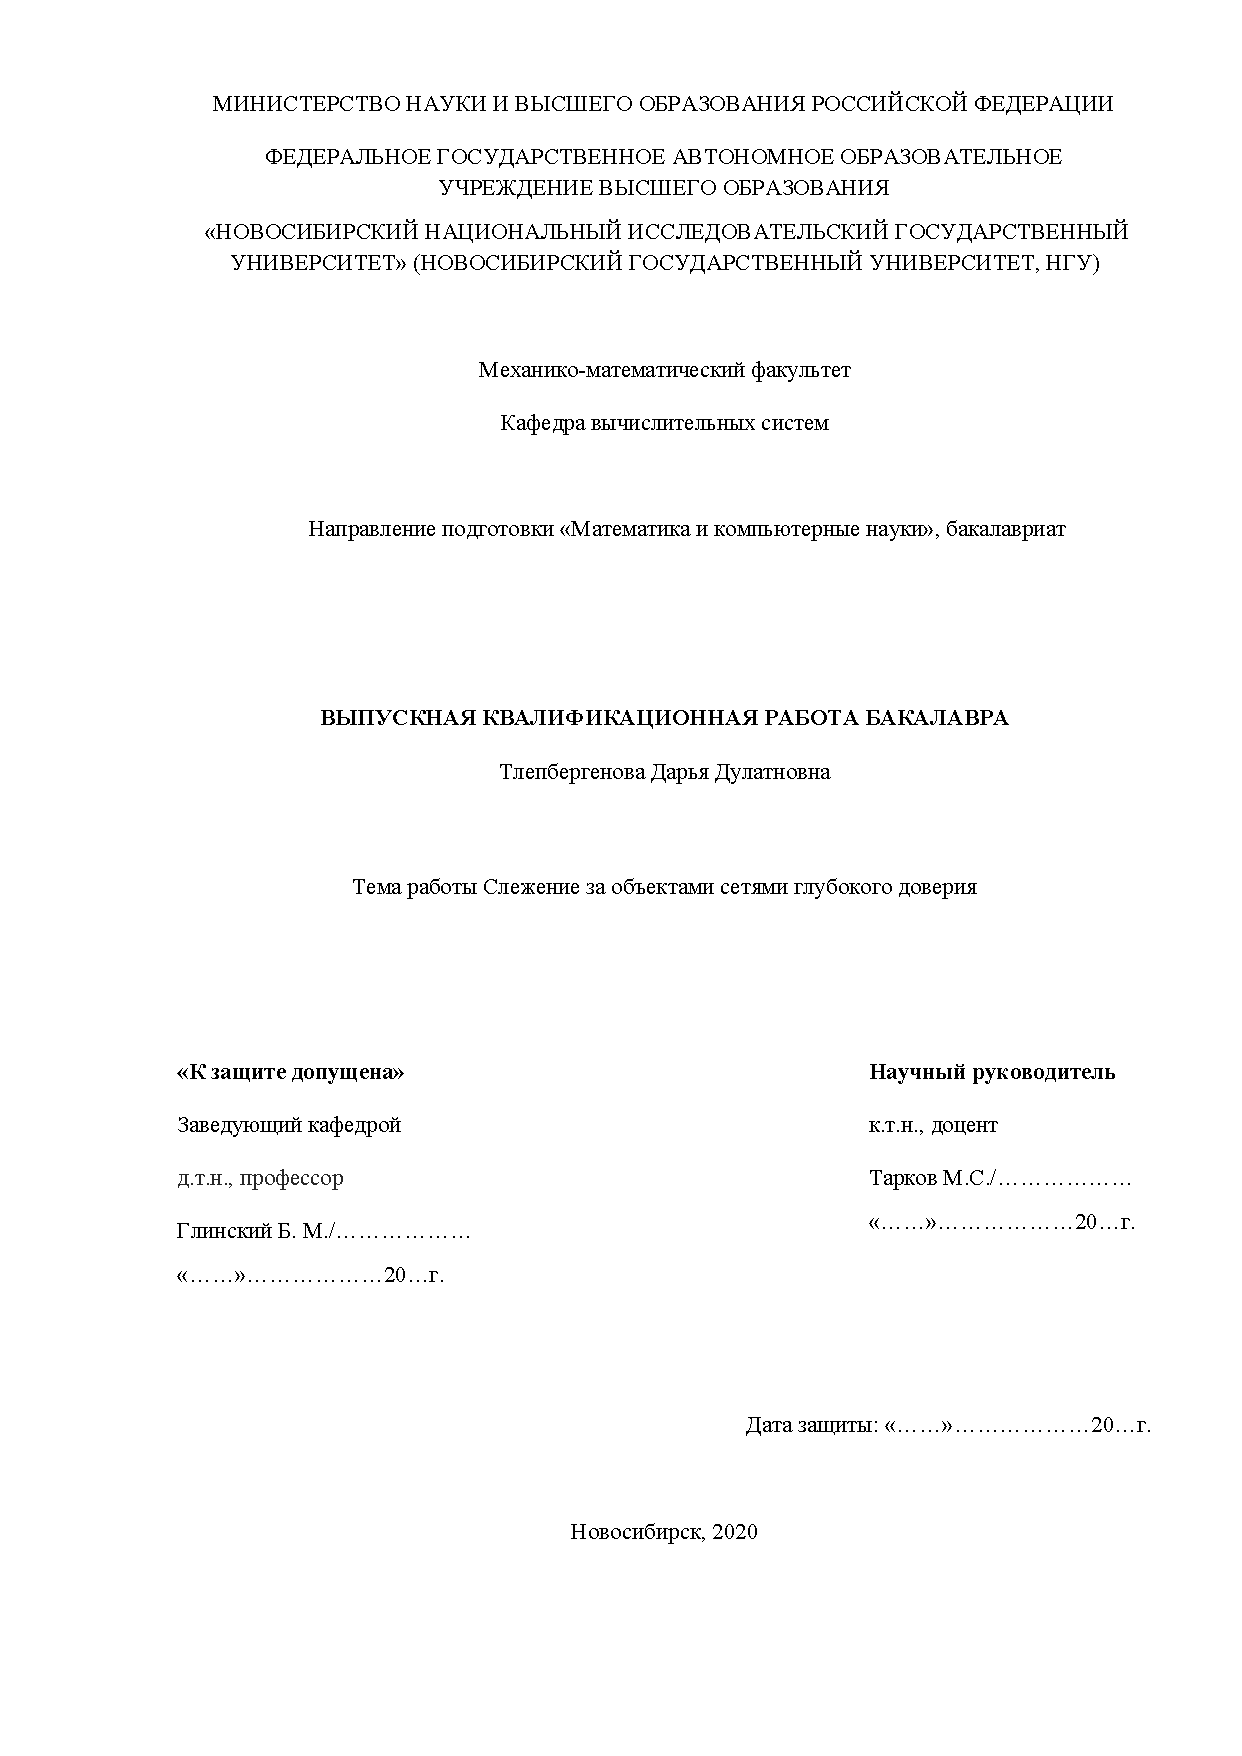
\includepdf[pages=-]{title_me.pdf}%титульный лист

\section*{Реферат}

\pagestyle{empty}
Название работы: Слежение за объектом сетями глубокого доверия.

Работа содержит 35 страниц, 10 иллюстраций, 3 таблицы, 10 источников, 5 приложений.

Ключевые слова: слежение за объектом, квантование весов, сеть глубокого доверия, число уровней квантования, нейрокомпьютерная сеть.

Объектом исследования является сеть глубокого доверия для слежения за объектом. 

Цель работы: исследование, разработка и модификация существующего алгоритма слежения за движущимся объектом на наборе изображений в режиме реального времени.

В ходе работы используется MATLAB версии R2019b9.7, исследуется выбранная сеть глубокого доверия DLT, применяется алгоритм квантования весовых коэффициентов матрицы и приводится аналитика влияния алгоритма на слежение за объектом. 

В результате получено число уровней квантования $L=128, 256$ необходимое для алгоритма квантования и приемлемого слежения. Также, зафиксировано уменьшение памяти в 10 раз для матрицы весовых коэффициентов.

Областью применения задачи слежения за объектом является навигация, видео-наблюдение, анализ движения и компьютерное зрение.
 % Вывод реферата

\newpage
\pagestyle{plain}
\tableofcontents % Вывод содержания
\setcounter{page}{2} 

\newpage
\section*{Введение}

\addcontentsline{toc}{section}{Введение}
Слежение за объектами -- одна из важных и интересных задач, применяемая во многих сферах жизни общества: в навигации, видео-наблюдении, анализе движения объекта, компьютерного зрения, аналитике спортивных видео материалов.  

В данный момент существует множество моделей слежения за объектами (их также называют трекерами), но не смотря на это, проблема точности, стабильности и быстродействия отслеживания все еще существует. Часто, возникают проблемы, связанные с отслеживанием в режиме реального времени, окклюзиями (затруднениями в разборе изображения), затемнением изображения, резкими движениями, изменениями освещения, уходом объекта из кадра, загромождением фона.

Многие, уже существующие методы решения, умеют неплохо справляться с возникающими проблемами, однако, они пользуются чрезмерным усложнением модели и требуют больших вычислений, из-за чего реализация в режиме реального времени становится затруднительной. Также, многие методы требуют больших затрат памяти для своей работы, в частности большее место для работы сети необходимо выделить для матрицы перехода или, как ее еще называют, матрицы весовых коэффициентов. Данные сведения подтверждают актуальность выбранной темы. 

Использование квантования весов в нейронной сети для изменения ее весовых коэффициентов  является одним из многочисленных решений проблемы, связанной с затратами памяти программной реализации. В свою очередь, данное внедрение делает актуальной задачу исследования влияния числа уровней квантования весов. 

Целью данной работы является исследование, разработка и модификация существующего алгоритма слежения за движущимся объектом на наборе изображений в режиме реального времени.

Задачи, которые были поставлены в данной работе:

\begin{itemize}[leftmargin=0em, itemindent=2.5 em,itemsep=1.5 pt,parsep=1.5 pt]
        \item[--] исследование существующих алгоритмов слежения за объектами; 
        \item[--] анализ существующего алгоритма сети глубокого доверия для слежения за конкретным объектом;
        \item[--] использование задачи квантования весовых коэффициентов на выбранной сети глубокого обучения;
        \item[--] реализация алгоритма квантования весов сети, которая является, в свою очередь, модификацией данной сети;
        \item[--] изучение влияния числа уровней квантования весовых коэффициентов;
        \item[--] изучение влияния квантования весов на алгоритм слежения за объектом.
\end{itemize}
 %Вывод введения

\newpage
\section*{Глава 1. Основные сведения и постановка задачи}
\addcontentsline{toc}{section}{Глава 1. Основные сведения и постановка задачи}
\setcounter{section}{1}

\subsection{Общие факты}

Глубокое обучение - это быстрорастущая часть машинного обучения, которая является подвидом искусственного интеллекта (ИИ), ставшая очень популярной в последние годы. Именно с помощью данного подхода, было разработано большое количество различных алгоритмов, связанных с компьютерным зрением, распознаванием речи, прогнозированием данных и другими сложными задачами [1].

Под глубокой сетью, в данном случае, подразумевается число слоев, через которые преобразуются данные. Таким образом, чем больше слоев в сети, тем глубже считается нейрокомпьютерная сеть. 

Глубокие нейронные сети стали хорошим решением, благодаря своим показателям в области признаков визуальной информации. В отличие от более простых конструкций, когда мы задаем признаки в ручную, многослойная архитектура может более эффективно описать исходный набор данных.

Одним из типов глубоких нейронных сетей являются сети глубокого доверия (ГСД). Данная модель нейронных сетей состоит из нескольких скрытых слоев, в каждом из которых нейроны не связаны между собой, но связаны с нейронами соседнего слоя. Таким образом, выполняя обучение на наборе примеров спонтанным образом, ГСД может обучаться и вероятностно отстраивать свои входы. Одна из таких моделей будет рассмотрена на задаче отслеживания траектории объекта.

Отслеживание объекта относится к автоматической оценке траектории при его перемещении на видео. Также отметим, что задача может требовать отслеживания нескольких объектов, но она все равно сводится к обработке каждого объекта в отдельности. Видео обычно представляется набором изображений. Помимо этого, может иметься набор значений к каждому изображению, которые задают действительное положение объекта. Второе используется для оценки работы данного алгоритма, чтобы оценить его точность и правильность в различных ситуациях.

После того, как отслеживаемый объект идентифицируется вручную или автоматически в первом видео-кадре, цель данного алгоритма состоит в том, чтобы автоматически вычислять траекторию движения объекта в последующих кадрах, то есть определять центр отслеживаемого объекта.

Большинство существующих моделей используют либо генеративный, либо дискриминационный подход. Генеративные модели, как и другие модели в машинном обучении с таким же понятием, предполагают, что отслеживаемый объект может быть описан некоторым генеративным процессом, и, следовательно, отслеживание заключается в поиске более вероятного кандидата среди, возможно, бесконечного множества. Так, например, генеративными моделями являются модели, описанные в статье [2].

С другой стороны, дискриминационный метод рассматривает данную задачу как проблему двоичной классификации, которая учится явно отличать отслеживаемый объект от его фона. К этой категории моделей относится online-трекер AdaBoost (OAB) [3].

В то время как генеративные методы обычно дают более точные результаты в менее сложных средах из-за более богатых представлений изображения, дискриминационные методы более устойчивы к сильным окклюзиям и вариациям, поскольку они явно учитывают фон [4].

В дальнейшем, в работе будут рассматриваться генеративные подходы к решению задачи слежения за объектами с помощью сетей глубокого доверия.

\subsection{Анализ существующих алгоритмов}

Рассмотрев уже существующие трекеры, например, описанные  в статьях [5] и [6], которые реализуют поставленную общую задачу отслеживания, нетрудно отметить их самый большой минус -- большие затраты на вычисление; они являются очень трудоемкими, объемными, что крайне не подходит, например, для онлайн-решения задачи.

Данное суждение приводит к поиску и аналитике альтернативных существующих алгоритмов. В ходе данной работы были рассмотрены следующие алгоритмы:

\begin{itemize}[leftmargin=0em, itemindent=2.5 em,itemsep=1.5 pt,parsep=1.5 pt]

\item[--] алгоритм глубокого обучения (DLT) и его программная реализация, описанная в статье [7]. Данный подход состоит из обучения с учителем глубокой сети, а затем онлайн-обучении во время непосредственного применения на конкретной последовательности. Именно данный алгоритм разбирается подробнее и на нем исследуется влияние квантования весов, по причине его хороших результатов в отслеживании объектов. Рассмотрим подробнее устройство данного алгоритма в следующих параграфах;

\item[--] алгоритм регионального глубокого обучения (RDLT), описанный в статье [8]. Данный алгоритм является своеобразным усложнением предыдущего. Взяв за основу схожие методы DLT, авторы усложнили его путем разделения целостной рамки, которая следит за объектом, на k частей;

\item[--] эталонный тест производительности [3], для сравнения существующих моделей между собой. В данной программе содержится 29 известных алгоритмов слежения, реализованных на основе оригинальных статей создателей методов, с одинаковыми  входными данными для чистоты эксперимента. В данную программу можно добавить модель, для сравнения, в частности в нее включена модель DLT.

\end{itemize}

Данная аналитика приводит нас к дальнейшему более подробному анализу работы алгоритма DLT, в частности его основных подходов и методов.

\subsection{Математическая модель DLT}
\subsubsection{Подход фильтр-частиц} 

Фильтр-частицы - частый генеративный подход к задаче отслеживания траектории движения. С точки зрения статистики, это последовательный метод выбора важности по методу Монте-Карло для оценки переменных скрытого состояния динамической системы на основе последовательности предыдущих наблюдений. Так, например, данный подход используется в реализации моделей DLT  и RDLT. Далее опишем основную идею данного метода.

Пусть $s^{t}$ и $y^{t}$ обозначают скрытое состояние и переменное наблюдение в момент времени $t$ (\ref{eq1}). Математически, отслеживание объекта, как мы уже говорили ранее, -- это задача о нахождении наиболее вероятного состояния для каждого временного шага t на основе наблюдений до предыдущего временного шага:

\begin{equation}\label{eq1}
    s^{t} = argmax(p(s^t|y^{1:t-1}))
\end{equation}

То есть, это такой аргумент функции вероятности в момент $t$ при условии предыдущих наблюдений, что функция на нем перенимает максимальное значение. После данной обработки, распределение переменной состояния обновляется в соответствии с правилом Байеса (\ref{baes}):

\begin{equation}\label{baes}
    p(s^t|y^{1:t}) = \dfrac{p(y^t|s^t)p(s^t|y^{1:t-1})}{p(y^t|y^{1:t-1})} 
\end{equation}

Исходя из формулы (\ref{baes}), аппроксимируем выражение слева с помощью набора $\{s^{(i)}_t\}^{n}_{i=1}$ дискретной конечной выборки, называемой частицами, с соответствующими весами (\ref{eq3}).

\begin{equation} \label{eq3}
    w^{(i)}_{t}=w^{(i)}_{t-1}\dfrac{p(y_t|s^{(i)}_t)p(s^{(i)}_t|s^{(i)}_{t-1})}{q(s_t|s_{1:t-1},y_{1:t})}
\end{equation}

В случае, если сумма весов меньше порогового значения, применяется повторная выборка, чтобы извлечь $n$ частиц из текущего набора частиц пропорционально их весу, а затем сбросить их веса до $\dfrac{1}{n}$. Если сумма весов превышает пороговое значение, применяется линейная нормализация, чтобы гарантировать, что сумма весовых коэффициентов равна 1. 

Для отслеживания объекта, переменная состояния $s_i$ обычно представляет собой шесть параметров аффинного преобразования: сдвиг, масштаб, соотношение сторон и поворот.

В частности, каждое измерение $q(s_t|s_{t-1})$ независимо моделируется нормальным распределением. Для каждого кадра результатом отслеживания является просто частица с наибольшим весом.

Структура фильтр-частиц является распространенным подходом в визуальном отслеживании. Она аппроксимирует распределение апостериорных состояний по множеству частиц, а не только по одной точке. Для визуального отслеживания это свойство облегчает модели восстановление после неверных результатов отслеживания.

\subsubsection{Предобработка данных}

Модель DLT представляет собой алгоритм, с помощью которого можно обработать в режиме реального времени последовательность изображений, определив на каждом из них центр отслеживаемого объекта. При поступлении изображений в модель, последовательность должна подать на вход программы вектор с координатами объекта на первом кадре (в пикселях), ширину и высоту объекта, и угол, на который повернут начальный объект. Также необходим аналогичный вектор с предполагаемым начальным сдвигом.

Далее производится нормализация данных, а именно ширина и высота отслеживаемого видео кадра приводится к разрешению 320 на 240, это нужно иметь ввиду при подаче последовательности в данный алгоритм. В случае если входная последовательность не находится в черно-белом формате она в него переводится, для уменьшения количества входных данных. Таким образом, мы можем напрямую использовать цветные изображения, при необходимости.

Также, для инициализации самой нейросети на нормализованных данных, необходимо загрузить обученные весовые коэффициенты сети. Данные матрицы были получены с помощью набора данных Tiny Images [9] -- вспомогательные данные для автономного обучения. Набор данных охватывает многие объекты и сцены, найденные в реальном мире. Из почти 80 миллионов крошечных изображений, каждое из которых имеет разрешение 32 × 32, случайным образом отобрали миллион изображений на которых было произведено обучение. На данном этапе в автономном режиме обучение выполняется путем шумоподовляющего автоэнкодера с накоплением (SDAE) для изучения общих характеристик в нем. Данная конструкция как раз относится к сетям глубокого доверия. Для более подробного описание этапа автономного обучения сети необходимо обратиться к статье [7].

\subsubsection{Онлайн обучение нейронной сети}

После произведенной пред-обработки данных, описанной выше, происходит этап онлайн обучения. Отметим сразу, что при выполнении данного, время работы сети заметно увеличивается, из-за дополнительного прохода по ней.

 \begin{figure}[h!]\label{arh}
    \centering
    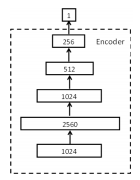
\includegraphics[width = 6 cm]{tests/img/online.PNG}
    \caption*{Рисунок 1.1 - Архитектура online-обучения DLT}
\end{figure}

Для первичного кадра последовательности происходит формирование 10 позитивных и 100 негативных примеров, на которых будет производиться онлайн обучение нейронной сети. Некоторые негативные примеры собраны из фона на небольшом расстоянии от объекта. Далее происходит инициализация сети, подгружается обученная матрица весовых коэффициентов. На основе полученных данных строится сигмоидальный классификационный слой, который добавляется в архитектуру SDAE (Рисунок 1.1), полученную в результате автономного обучения.

Базовым строительным блоком SDAE является однослойная нейрокомпьютерная сеть, которая называется автоинкодером с шумоподавлением (DAE). Она является более поздним вариантом обычного автоэнкодера и учится восстанавливать образец данных из его поврежденной версии. 

После этого, для вычисления коррекции весовых коэффициентов матрицы, выполняется алгоритм обратного распространения ошибки, после чего завершается этап инициализации нейронной сети.

Кроме того, стоит добавить, что когда считывается новый видео-кадр, сначала вычисляются фильтр-частицы в соответствии с подходом, описанным выше, а затем достоверность каждой частицы определяется путем простого прямого прохода через сеть. 

\subsection{Квантование весов}

Известно, что реализация нейронной сети задействует много памяти для хранения, как минимум, матрицы весов для каждого слоя нейронов. Так как рассматривается глубокое обучение -- множество матриц перехода, из-за чего хранение является дорогостоящей опцией.

Данную проблему можно решить с помощью использования вместо ячейки памяти - мемристора. Задача квантования весов, описанная в статье [10], которая является ключевой в данной работе, использует их для аппаратной реализации весов нейронной сети. Многоуровневые мемристоры реализуют множество дискретных уровней проводимости (иначе говоря, значение мемристора может принимать L значений числа уровней квантования). Они основаны на механизме переключения, а также, достаточно широко распространены, в отличие от аналоговых мемристоров с непрерывной проводимостью. В настоящей работе, необходимо отметить, что многоуровневые мемристоры устойчивы к различным статистическим отклонениям по сравнению с аналоговыми. 

% Перевод данных об алгоритмах
	\renewcommand{\listalgorithmname}{Список алгоритмов}
	\floatname{algorithm}{Алгоритм}
	
	% Перевод команд псевдокода
	\algrenewcommand\algorithmicwhile{\textbf{До тех пока}}
	\algrenewcommand\algorithmicdo{\textbf{выполнять}}
	\algrenewcommand\algorithmicrepeat{\textbf{Повторять}}
	\algrenewcommand\algorithmicuntil{\textbf{Пока выполняется}}
	\algrenewcommand\algorithmicend{\textbf{Конец}}
	\algrenewcommand\algorithmicif{\textbf{Если}}
	\algrenewcommand\algorithmicelse{\textbf{иначе}}
	\algrenewcommand\algorithmicthen{\textbf{тогда}}
	\algrenewcommand\algorithmicfor{\textbf{Цикл}}
	\algrenewcommand\algorithmicforall{\textbf{Выполнить для всех}}
	\algrenewcommand\algorithmicfunction{\textbf{Функция}}
	\algrenewcommand\algorithmicprocedure{\textbf{Процедура}}
	\algrenewcommand\algorithmicloop{\textbf{Зациклить}}
	\algrenewcommand\algorithmicrequire{\textbf{Условия:}}
	\algrenewcommand\algorithmicensure{\textbf{Обеспечивающие условия:}}
	\algrenewcommand\algorithmicreturn{\textbf{Возвратить}}
	\algrenewtext{EndWhile}{\textbf{Конец цикла}}
	\algrenewtext{EndLoop}{\textbf{Конец зацикливания}}
	\algrenewtext{EndFor}{\textbf{Конец цикла}}
	\algrenewtext{EndFunction}{\textbf{Конец функции}}
	\algrenewtext{EndProcedure}{\textbf{Конец процедуры}}
	\algrenewtext{EndIf}{\textbf{Конец условия}}
	\algrenewtext{EndFor}{\textbf{Конец цикла}}
	\algrenewtext{BeginAlgorithm}{\textbf{Начало алгоритма}}
	\algrenewtext{EndAlgorithm}{\textbf{Конец алгоритма}}
	\algrenewtext{BeginBlock}{\textbf{Начало блока. }}
	\algrenewtext{EndBlock}{\textbf{Конец блока}}
	\algrenewtext{ElsIf}{\textbf{иначе если }}
	
	\begin{algorithm}[h!]
		\begin{algorithmic}[1]
			\State Находим максимальный по модулю элемент матрицы весов $W_{max}$
			\State $\Delta = \frac{W_{max}}{L-1}$
			\For{ по всем элементам $W_{ij}$}
			\For{\textbf{от} $k=0$ \textbf{до} L}
			\If{$(k-1) \Delta < |W_{ij}| < k \Delta$}
			\State $W{ij} = (k-1) \Delta sign(W_{ij})$
			\EndIf
			\EndFor
			\EndFor
		\end{algorithmic}
	\caption*{Алгоритм 1.1 -- Алгоритм квантования весовых коэффициентов}
	\end{algorithm}
	
Для реализации задачи квантования необходимо после пред-обучения нейронной сети и заполнения матрицы весов, при запуске частного случая, а именно после загрузки весов обученной сети, провести квантование данной матрицы. Алгоритм квантования весов (Алгоритм 1.1) заключается в замене весовых коэффициентов матрицы на аппроксимированные значения в зависимости от уровней квантования. 

Для квантования весов необходимо также определиться с числом уровней квантования. Поиск данного числа предлагается искать опытным путем через сравнение с исходными значениями алгоритма слежения. 
 %Вывод 1 главы

\newpage
\section*{Глава 2. Реализация и тестирование}
\addcontentsline{toc}{section}{Глава 2. Реализация и тестирование}

\setcounter{section}{2}
\setcounter{subsection}{0}

\subsection{Реализация}
 Для реализации алгоритма DLT был использован MATLAB версии R2019b 9.7. Язык MATLAB - является высокоуровневым, имеет широкий спектр функций, интегрированную среду разработки, объектно-ориентированные возможности и интерфейсы к программам. Также, в нем имеются такие наборы инструментов, как Neural Network Toolbox и различные математические пакеты, удобные для вычисления сложных алгоритмов.
 
 \begin{figure}[h]
    \label{car4}
    \centering
    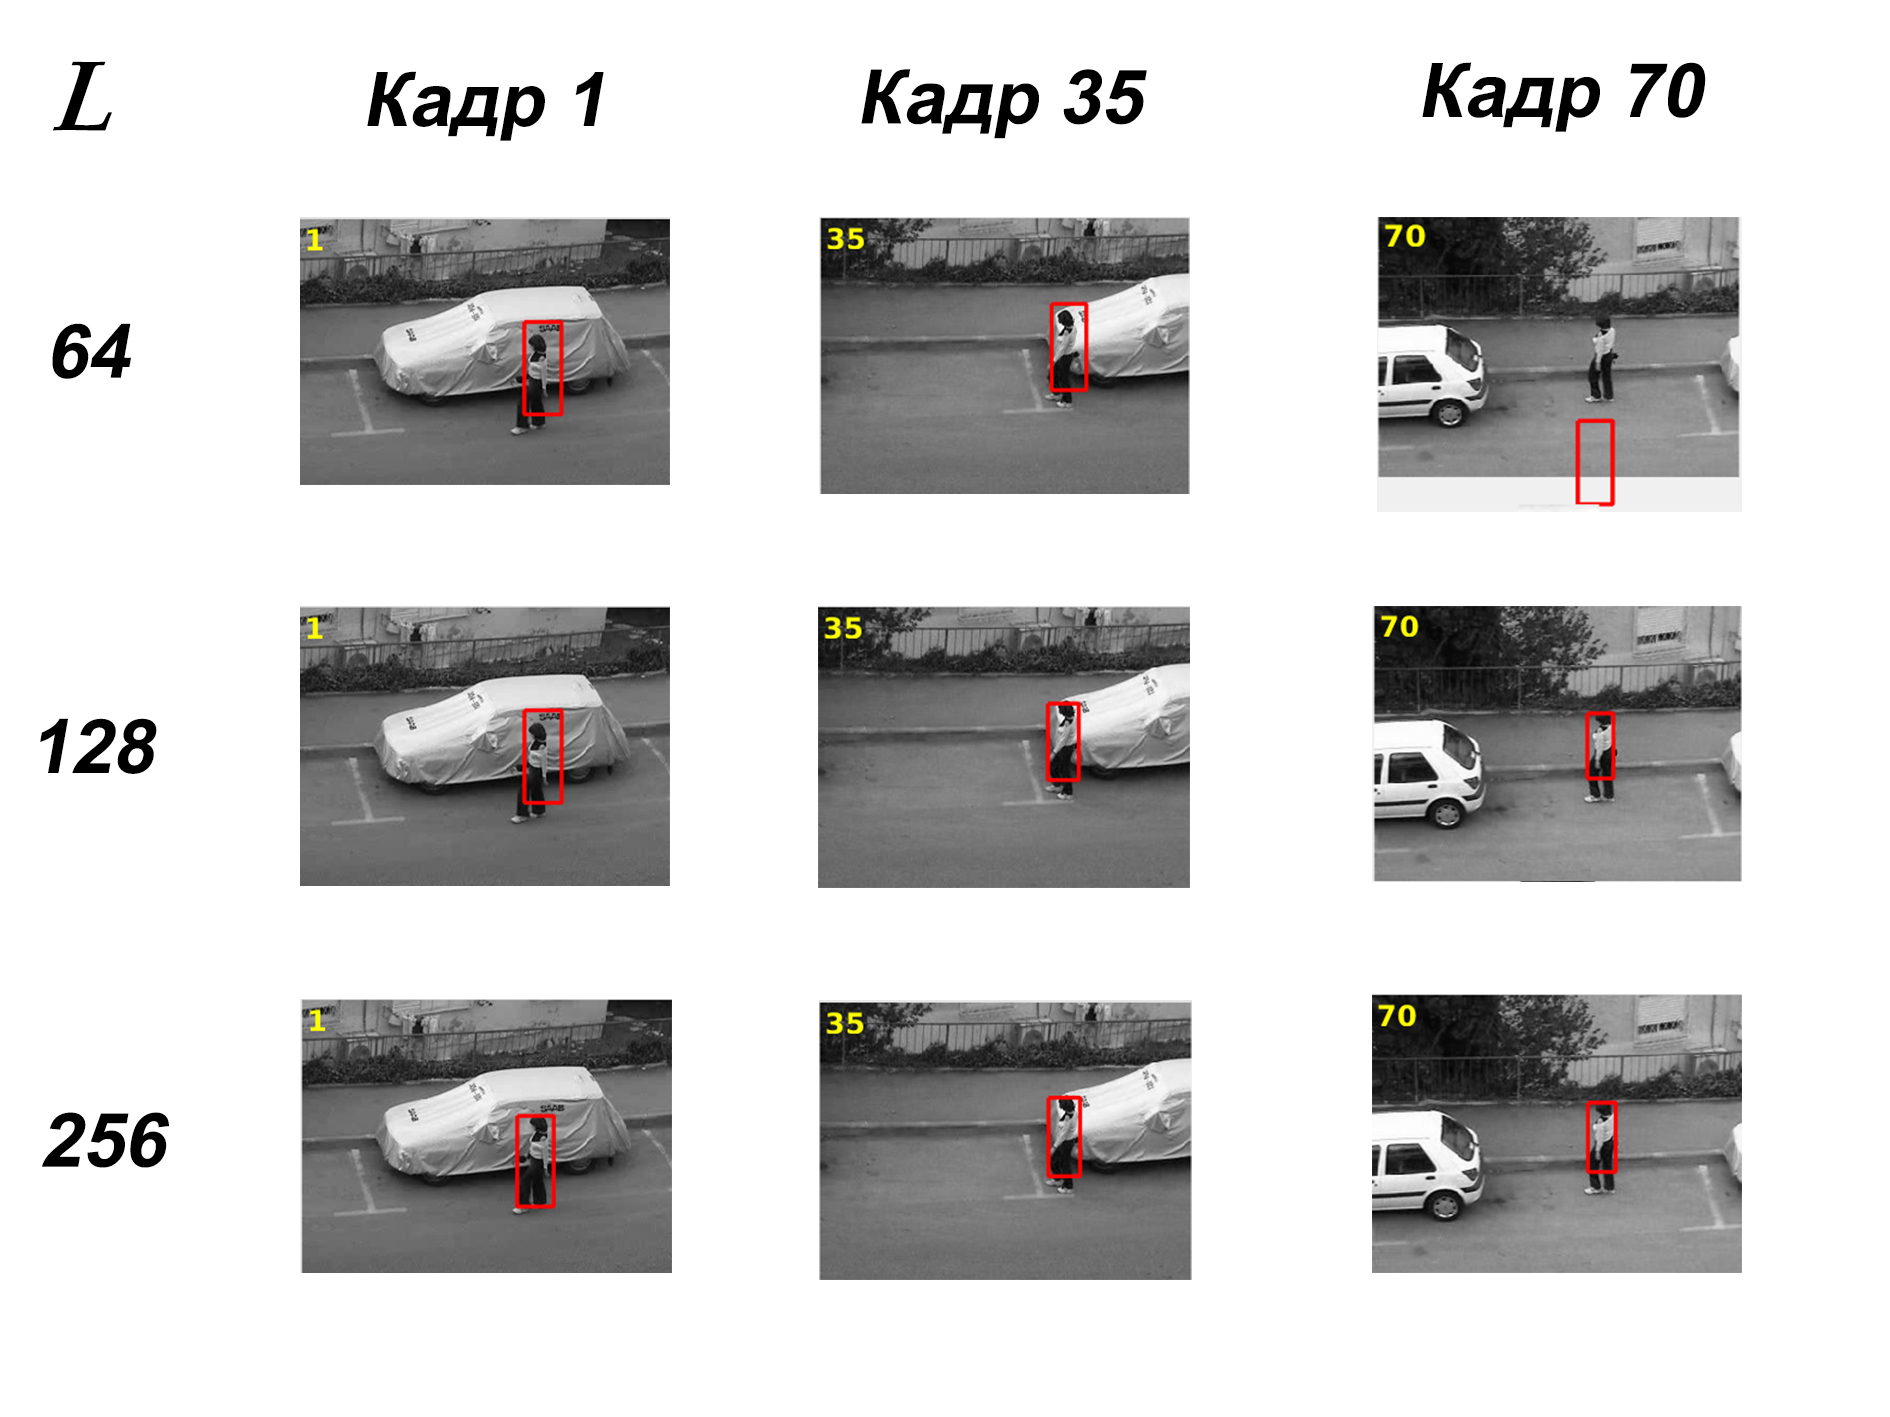
\includegraphics[width=10cm]{tests/img/Bez_imeni-2.jpg}
    \caption*{Рисунок 2.1 - Использование DLT на примере видео car4}
\end{figure}
 
 Также, можно наблюдать работу данной программы в режиме реального времени, наблюдая на экране по-кадровый вывод на котором красной рамкой демонстрируется траектория объекта, подсчитанная с помощью алгоритма DLT. На рисунке (2.1) мы можем наблюдать работу этой программы для конкретной последовательности car4.
 
 Для использования DLT необходимо изменить путь к папке с изображениями, которые мы хотим протестировать с помощью данного алгоритма в файле run\_individual.m и запустить его. На экране начнет появляться по-кадровая работа данного алгоритма. 
 
\subsection{Эксперименты}
\subsubsection{Входные данные}
В качестве входного набора изображений для тестирования оригинального и квантованного алгоритма, были использованы наборы изображений [4], разработанные специально для тестирования подобных моделей. В данной работе присутствует $50$ экземпляров видео, представленных в виде последовательности изображений, которые можно использовать для тестирования подобных программ слежения за объектами. 

В каждом наборе содержится последовательность кадров целостного видео в формате jpg или png, к которым прилагается файл. В данном файле присутствует таблица, содержащая в первом и втором столбце - координаты левого нижнего края объекта сначала по горизонтали, затем по вертикали соответственно; в третьем и четвертом - ширину и длину отслеживаемого объекта. С его помощью несложно определить точные координаты центра рамки и границ объекта для сравнения с полученными результатами.

За образцовый набор кадров были выбраны первые 70 кадров из последовательности Woman. Следует обратить внимание, что необходимо выбрать последовательность, которая будет хорошо работать на выбранном трекере. В силу того, что в экземплярах последовательностей, описанных ранее, в основном присутствуют образцы с определенными затруднениями, такие как: попадание объекта в тень или заходящим за какой либо объект, выходом за пределы кадра или со сложным фоном, специально для тестирования моделей в сложных ситуациях. Из всех данных видеоматериалов, был выбран стабильный участок последовательности, по причине исследования именно алгоритма квантования.

Тестирование проводилось с помощью процессора Intel(R) Pentium(R) CPU 2020M 2.40GHz. Заметим сразу, что вычисления можно ускорить, если вычисления проводить с помощью GPU и MATLAB Parallel Computing Toolbox, как для автономного обучения или квантования, так и для online-отслеживания.

\subsubsection{Реализация алгоритма квантования}

Необходимо выполнить квантование обученной матрицы весовых коэффициентов до начала работы онлайн обучения. Соответственно, для этого нужно выполнить алгоритм квантования весов и сохранить полученные результаты, для того чтобы в дальнейшем данные матрицы подгружались уже с квантованными весами. Также, следует квантовать веса с разным числом уровней квантования, для определения подходящего к данному трекеру числа и аналитике влияния этого числа на алгоритм.   

\begin{figure}[h!]
    \centering
    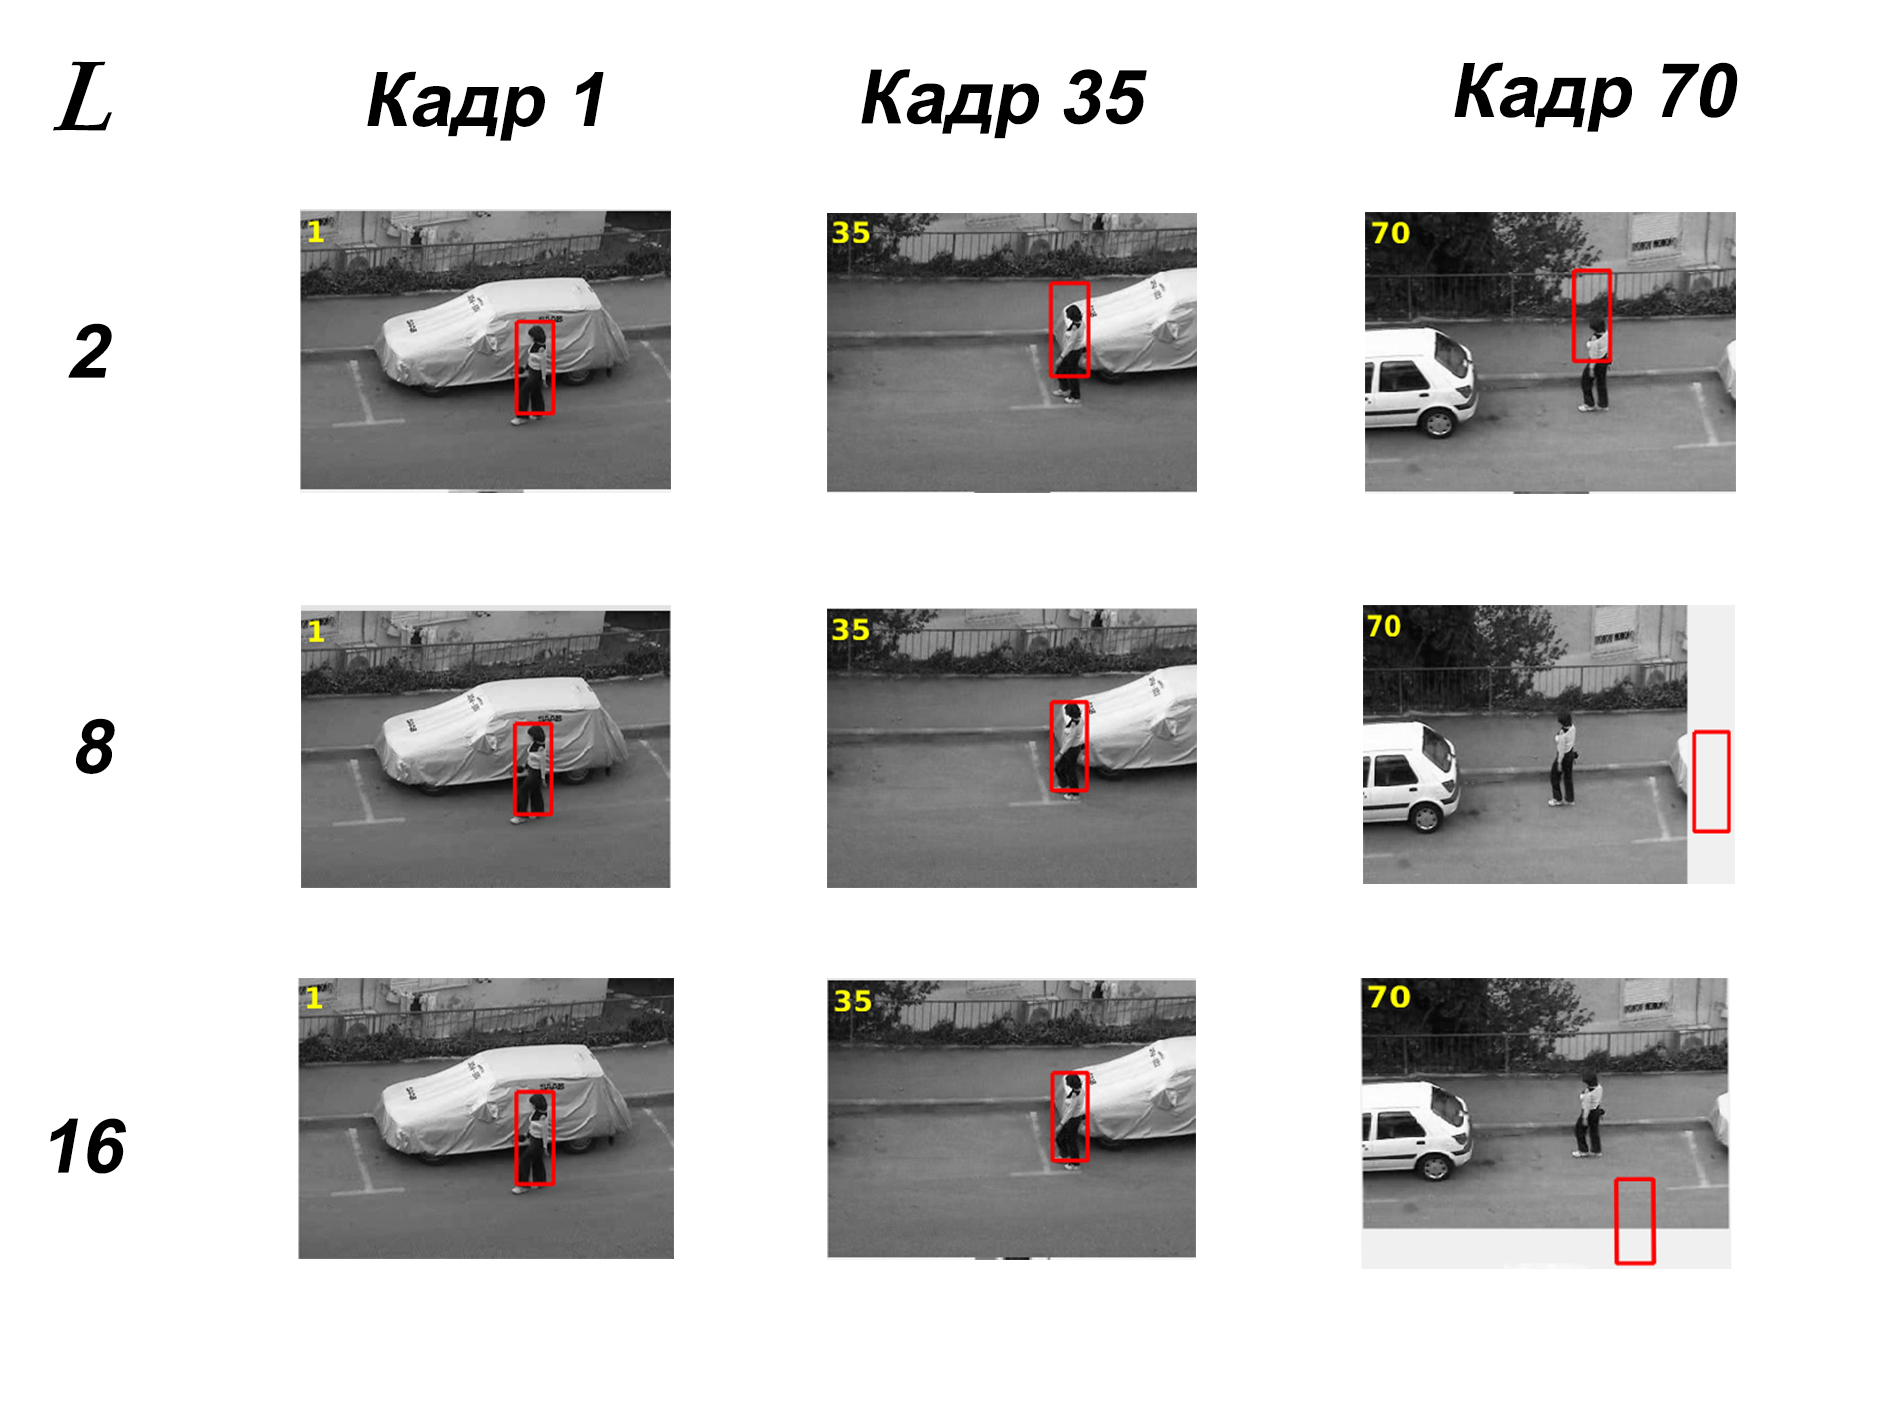
\includegraphics[width = 14 cm]{tests/img/Bez_imeni-1.jpg}
    \caption*{Рисунок 2.2 -- Работа алгоритма слежения. L - число уровней квантования}
\end{figure}

На основе вышеупомянутого, был реализован алгоритм квантования весовых коэффициентов сети (Приложение 1). Данный алгоритм запускается с разным значением параметра, отвечающего за число уровней квантования. Для определенности были выбраны следующие значения числа уровней квантования $L = 2,4,8,16,32,64,128,256$. В результате чего получаются наборы  данных, которые в последующем, вместо данного алгоритма, подгружаются на место весовой матрицы. Это необходимо для сокращения времени работы алгоритма и также для чистой оценки времени работы именно отслеживающего алгоритма.

\begin{table}[h!]
\caption*{Таблица 2.1 -- Значения памяти в зависимости от уровня квантования}
\begin{tabular}{|c|c|c|c|c|c|c|c|c|}
\hline
L                                                       & 2    & 4    & 8    & 16   & 32   & 64   & 128 & 256  \\ \hline
\begin{tabular}[c]{@{}c@{}}память\\ (в MB)\end{tabular} & 1.5 & 1.5 & 1.5 & 1.5 & 1.6 & 1.8 & 2.1  & 2.8\\ \hline
\end{tabular}
\end{table}

Память, занятая матрицами после выполнения алгоритма квантования, в зависимости от числа уровней квантования, представлена выше (Таблица -- 2.1). Заметим, что исходные весовые матрицы занимали 21MB, а получившиеся в результате квантования матрица, например при $L=128$ занимает 2.1 MB памяти, что в 10 раз лучше изначальных данных. 

\begin{figure}[h!]
    \centering
    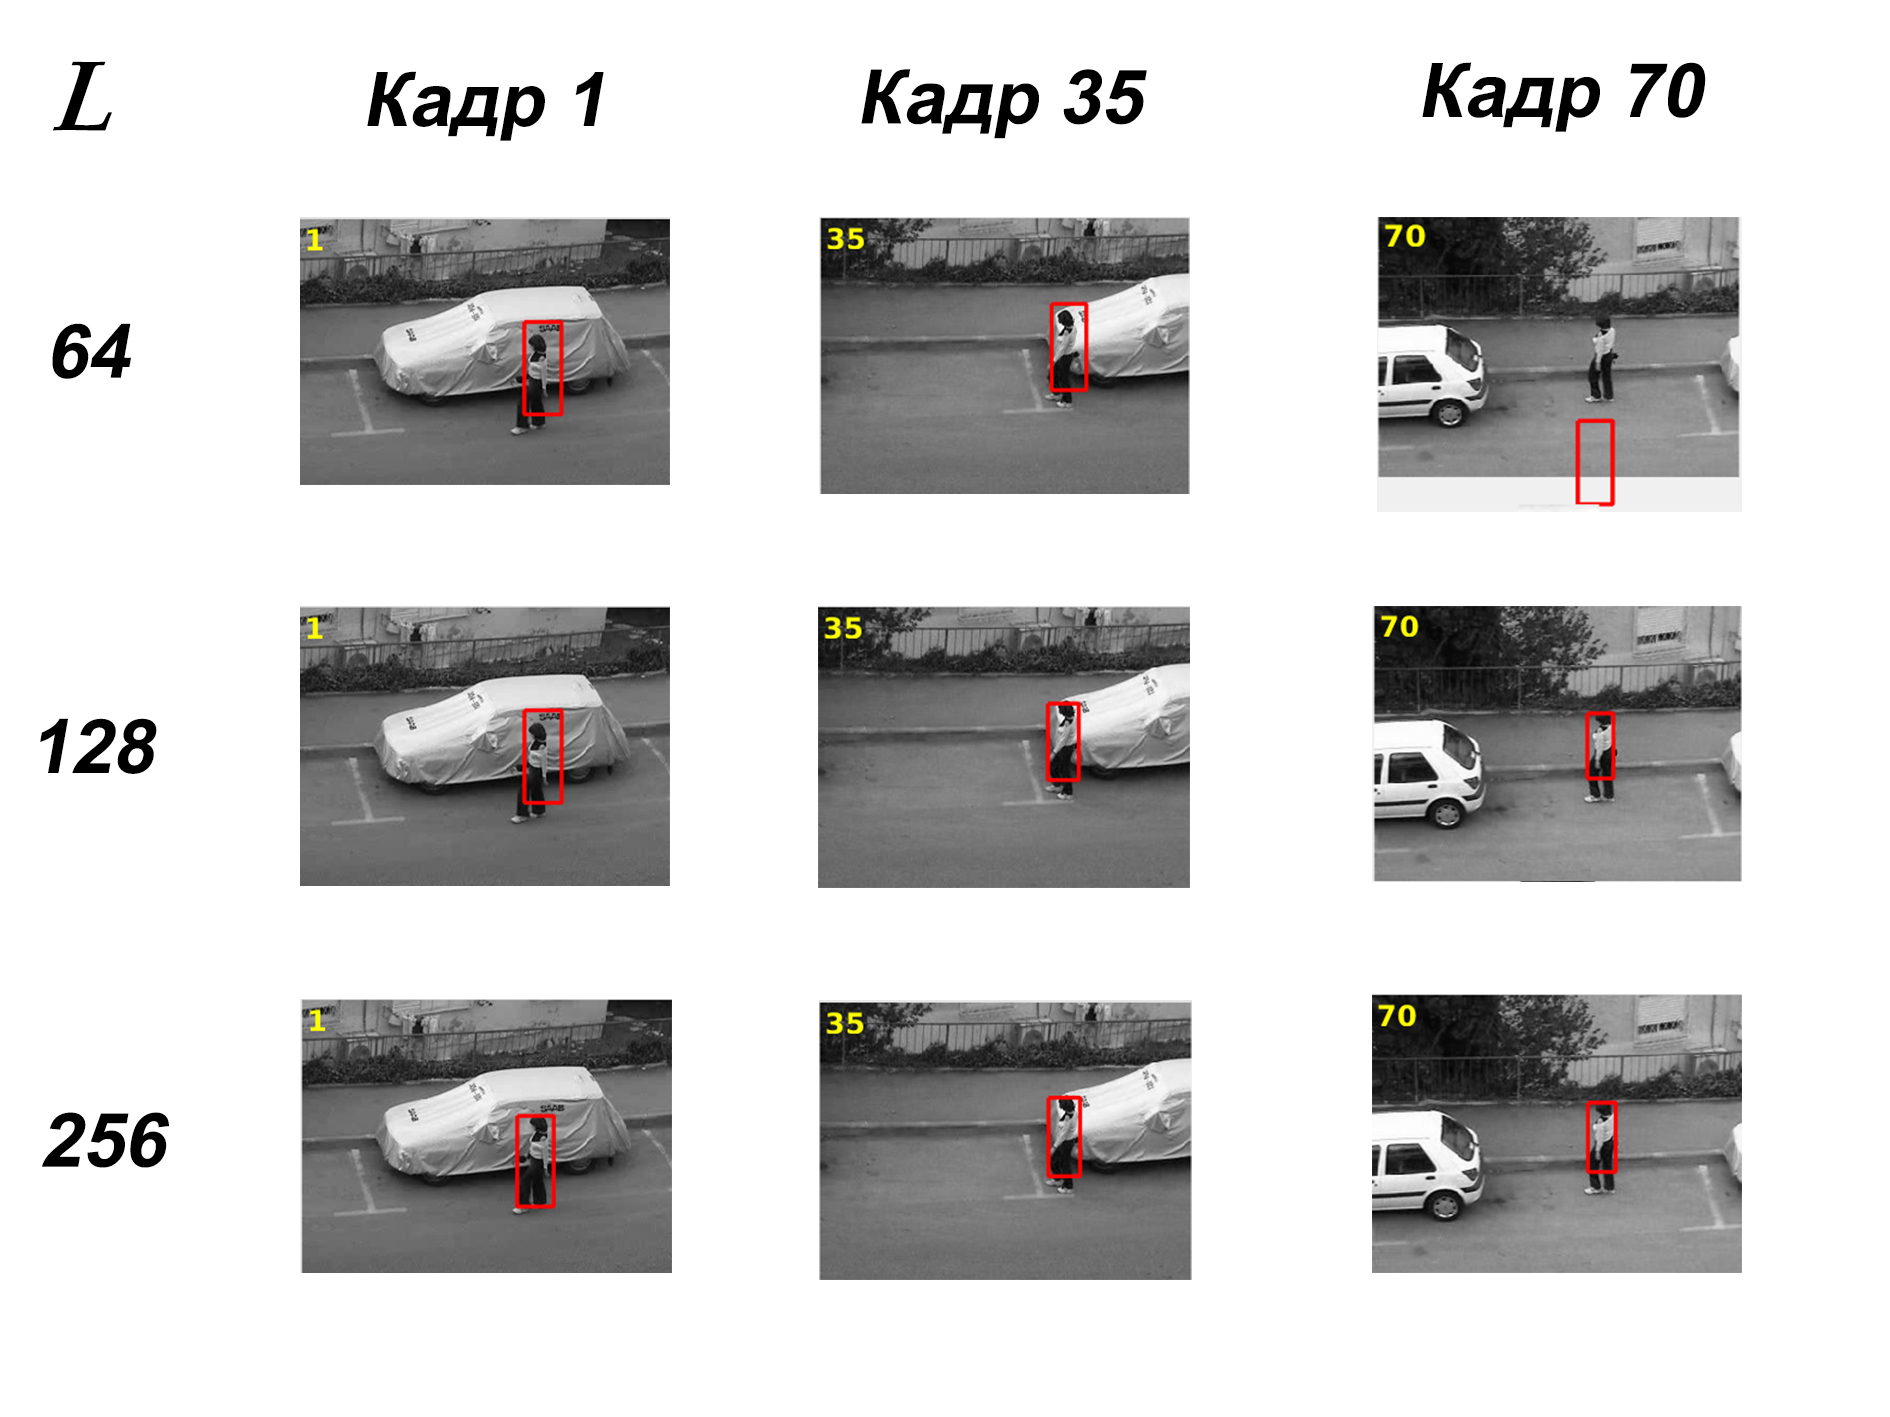
\includegraphics[width = 14 cm]{tests/img/Bez_imeni-2.jpg}
    \caption*{Рисунок 2.3 -- Работа алгоритма слежения. L - число уровней квантования}
\end{figure}

Таким образом, данный алгоритм запускается с разными квантованными матрицами, то есть матрицы с разным числом уровней квантования и на основе полученных результатов строится дальнейшая аналитика (Рисунок 2.2, 2.3). 

\subsubsection{Влияние квантования на время работы алгоритма}

Рассмотрим как меняется время работы алгоритма отслеживания с квантованными весовыми коэффициентами. Отметим, что время работы очень зависит от устройства, на котором запускается данная программа, и его параметров. В начале, мы зафиксируем время работы оригинального алгоритма слежения. Алгоритм DLT на выбранной последовательности без квантования весов работал в течение 47.51 секунд и с $fps = 1.47$ кадров в секунду. Далее, мы будем фиксировать три параметра для квантованного запуска программы - это общее время работы алгоритма отслеживания, количество кадров в секунду во время работы алгоритма и время, затраченное на квантование матриц.

Зависимость времени работы программы слежения от числа уровней квантования L представлена ниже (Таблица 2.2). По данной таблице мы можем наблюдать уменьшение времени работы алгоритма отслеживания от числа уровней квантования. 

\begin{table}[h!]
\caption*{Таблица 2.2 -- Зависимость времени от числа уровней квантования}
\begin{tabular}{|c|c|c|c|}
\hline
L   & \begin{tabular}[c]{@{}c@{}}Время работы\\  программы\end{tabular} & \begin{tabular}[c]{@{}c@{}}Количество кадров\\  в секунду (fps)\end{tabular} & \begin{tabular}[c]{@{}c@{}}Время квантования\\   матриц\end{tabular} \\ \hline
2   & 75.4                                                              & 0.93                                                                         & 10.2                                                                 \\ \hline
4   & 73.8                                                              & 0.95                                                                         & 10.1                                                                 \\ \hline
8   & 74.6                                                              & 0.94                                                                         & 12.3                                                                 \\ \hline
16  & 72.6                                                              & 0.96                                                                         & 18.6                                                                 \\ \hline
32  & 72.6                                                              & 0.96                                                                         & 30.1                                                                 \\ \hline
64  & 74.6                                                              & 0.94                                                                         & 54                                                                   \\ \hline
128 & 45.7                                                              & 1.53                                                                         & 105.3                                                                \\ \hline
256 & 43.9                                                              & 1.6                                                                          & 202                                                                  \\ \hline                     
\end{tabular}
\end{table}

При $L = 2,4,..,64$ значительных изменений во времени не наблюдается. Худший результат наблюдается при $L=2$. Во время работы алгоритма при таких значениях уровня квантования наблюдается слишком частое подобучение, то есть происходит онлайн обучение сети на конкретном кадре, в следствие чего время работы по сравнению с непрерывными весами увеличивается. При $L = 128$ и $L = 256$ время алгоритма схоже с оригинальным значением времени.

Количество кадров в секунду берется в среднем за все время работы алгоритма. Наблюдается уменьшение данного показателя при подобучении, увеличение при его отсутствии, и, также, как и параметр общего времени, с увеличением числа уровней квантования количество кадров в секунду растает.

Время квантования матриц, начиная от $L=8$ растет линейно, относительно числа уровней квантования. Другими словами, время квантования увеличивается примерно в 2 раза при увеличении числа уровней квантования в 2 раза. Это наблюдается в силу одного вхождения цикла по L в реализацию алгоритма квантования. 

Для большей наглядности, для полученных данных была реализована диаграмма (Рисунок 2.4). С ее помощью можно наблюдать динамику изменения времени относительно числа уровней квантования и сравнение с изначальным значением времени. 

\begin{figure}[h!]
    \centering
    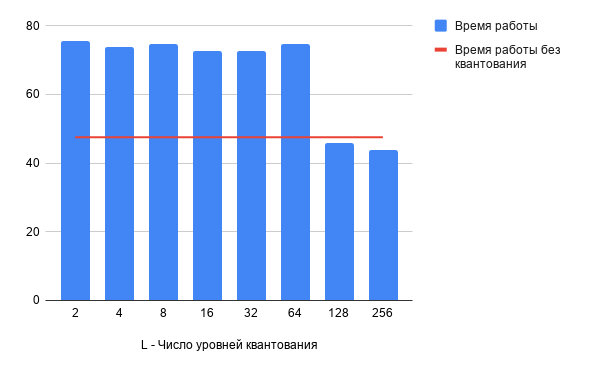
\includegraphics[width = 14 cm]{tests/img/time.png}
    \caption*{Рисунок 2.4 -- Зависимость времени от числа уровней квантования }
    \label{fig:my_label}
\end{figure}

Таким образом, из данного рассуждения следует, что лучшие результаты достигнуты с точки зрения времени при $L = 128, 256$, наихудшие -- при $L=2$.

\subsubsection{Влияние квантования на смещение центра}

Для определения смещения центра объекта алгоритмом, необходимо снять координаты перемещения для него с неквантованными весовыми коэффициентами. Сначала, вычисляются координаты смещения для исходного алгоритма DLT. Далее, снимаются аналогичные координаты, но уже после квантования весов для различных уровней квантования, и определяется модуль разницы между исходным алгоритмом и модифицированным. Таким образом, получается смещение, которое может показывать качество работы алгоритма слежения за объектами.

\begin{figure}[h!]
    \centering
    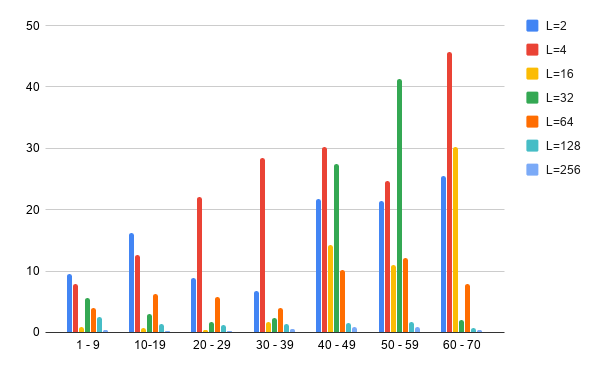
\includegraphics[width = 14 cm]{tests/img/diag_x.png}
    \caption*{Рисунок 2.5 -- Смещение центра по горизонтали от числа уровней квантования}
    \label{fig:my_label}
\end{figure}

В результате данной работы были определены смещения центра объекта для следующих чисел уровней квантования $L = 2, 4, 16, 32, 128, 256$. Работая с координатами центра рамки, все вычисления разделяются  на значения по горизонтали и вертикали. Полученные данные были занесены в таблицы сначала относительно горизонтальной координаты (Приложение 2).

Также, выше представлен рисунок, полученный на основе данной таблицы, для более наглядного представления относительно большого объема данных (Рисунок 2.5).

\begin{figure}[h!]
    \centering
    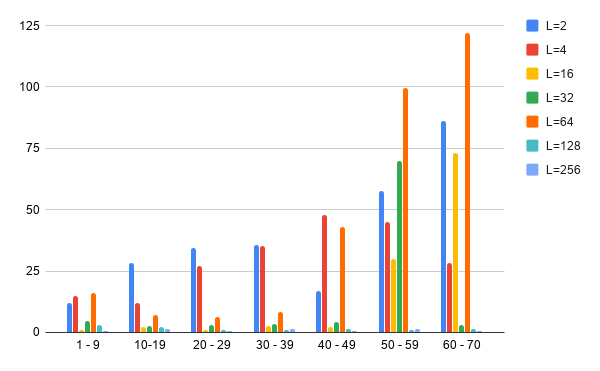
\includegraphics[width = 13 cm]{tests/img/diag_y.png}
    \caption*{Рисунок 2.6 -- Смещение центра по вертикали от уровней квантования}
    \label{fig:my_label}
\end{figure}

Такие подробные данные позволяют покадрово определить в каких именно изображениях ухудшается слежение. Так, например, можно заметить сильное смещение в последних кадрах последовательности при $L=4$.

Полученные рассуждения можно повторить и для вычисления смещения центра рамки по вертикали (Приложение 3) и аналогично рассмотреть полученные результаты на рисунке (Рисунок 2.6). По данному рисунку видно, что также как и по горизонтали, здесь наблюдается усиление смещения к концу последовательности. 

\begin{table}[h!]
\caption*{Таблица 2.3 -- Зависимость смещения центра от числа уровней квантования}
\begin{tabular}{|c|c|c|}
\hline
\multirow{2}{*}{L} & \multicolumn{2}{c|}{\begin{tabular}[c]{@{}c@{}}Среднее смещение\end{tabular}}                                                                      \\ \cline{2-3} 
                   & \begin{tabular}[c]{@{}c@{}}по горизонтали (по координате x)\end{tabular} & \begin{tabular}[c]{@{}c@{}}по вертикали (по координате y)\end{tabular} \\ \hline
2                             & 16,2                                   & 41,9                                 \\ \hline
4                             & 24,4                                   & 30,2                                 \\ \hline
8                             & 41                                     & 7,6                                  \\ \hline
16                            & 8,4                                    & 17                                   \\ \hline
32                            & 11,8                                   & 13                                   \\ \hline
64                            & 7,2                                    & 44,7                                 \\ \hline
128                           & 1,6                                    & 1,6                                  \\ \hline
256                           & 0,5                                    & 0,9                                  \\ \hline
\end{tabular}
\end{table}

По данным относительно каждого кадра исследуемой последовательности, необходимо сделать усреднение, чтобы определить качество работы данного алгоритма для каждого уровня квантования в среднем. Полученные данные занесены в таблицу зависимости среднего смещения центра рамки захвата (в пикселях) от числа уровней квантования (Таблица 2.3).

Из полученных данных наблюдается уменьшение ошибки с увеличением числа уровней квантования, после значения $L=64$. При $L = 128$  b $L=256$ для смещений происходит существенное уменьшение данного параметра. Таким образом, можно выбрать какое смещение будет наиболее приемлемо. Наихудшее среднее смещение наблюдается как при $L=2$, так и при $L=64$, а при $L=256$ -- наилучшее. При этом, можно отметить, что значения при $L=128$  вполне приемлемы, хотя временные затраты на реализацию и объем памяти меньше, чем у лучшего кандидата.     

\begin{figure}[h!]
    \centering
    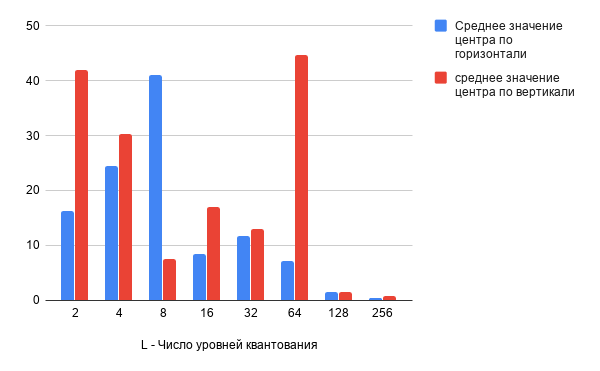
\includegraphics[width = 14 cm]{tests/img/sm.png}
    \caption*{Рисунок 2.7 -- Зависимость смещения центра от числа уровней квантования}
\end{figure}

Далее, проиллюстрируем таблицу, упомянутую выше, с помощью столбчатой диаграммы, изображенной на рисунке (Рисунок 2.7). На ней заметна разница между средним смещением центра рамки по вертикали и по горизонтали. 

По полученным данным смещения и среднего смещения центра отслеживающей рамки отчетливо видны слишком большие изменения (как в последних кадрах) и незначительные, близкие к исходному (как при $L=128,256$). В дополнении к этому, хотелось бы проанализировать для каждого кадра, теряет ли трекер отслеживаемый объект. Другими словами, насколько значительно 
полученное смещение для отслеживания выбранного объекта. Данный анализ можно произвести зрительно, с помощью выводимых кадров во время работы программы, но данный способ не надежен и имеет субъективный характер.

Для получения желаемых результатов, вычисляется относительное смещение в зависимости от числа уровней квантования. Для вычисления данных параметров необходимо полученные выше смещения центра рамки относительно каждого кадра разделить (в случае горизонтальной координаты) на ширину соответствующего кадра последовательности. Полученные результаты представлены в виде таблицы (Приложение 4). Из данной таблицы следует, что вплоть до $L=64$, отслеживание объекта по горизонтали происходит с потерей объекта, при $L=128$ -- ни в одном кадре не теряется объект, а при $L=256$ -- остается достаточно мало кадров, в которых смещение отлично от нуля. 

\begin{figure}[h!]
    \centering
    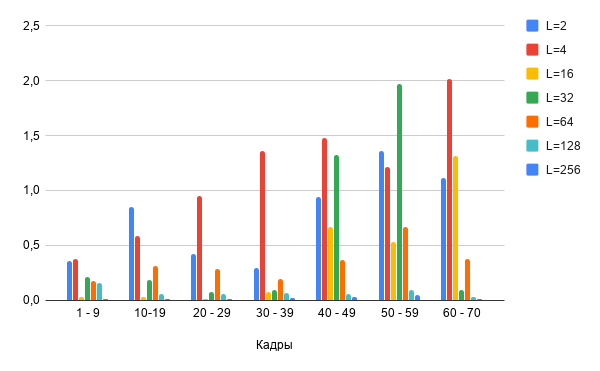
\includegraphics[width = 14 cm]{tests/img/diag_rlt_disp_x.png}
    \caption*{Рисунок 2.8 -- Относительное смещение (горизонталь) от уровней квантования}
\end{figure}

По полученной таблице была реализована диаграмма, изображенная на рисунке (Рисунок 2.8). Аналогичные рассуждения можно провести и для смещений центра рамки по вертикали, в данном случае разделив соответствующие смешения на соответствующую длину (Приложение 5). 

\begin{figure}[h!]
    \centering
    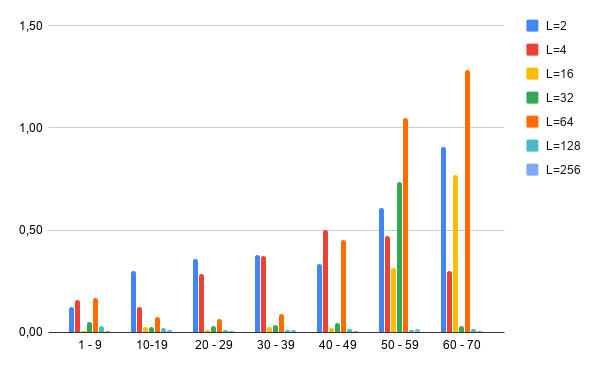
\includegraphics[width = 14 cm]{tests/img/diag_rlt_disp_y.png}
    \caption*{Рисунок 2.9 -- Относительное смещение (вертикаль) от уровней квантования}
\end{figure}

На иллюстрации вертикального относительного смещения (Рисунок 2.9), в отличие от горизонтального, наблюдается иные результаты. При $L = 2,4,..,64$ показатели превышают 1, что свидетельствует о потери объекта алгоритмом отслеживания. Но не смотря на это, при $L = 128,256$ ни в одном кадре не теряется объект.

В результате данных экспериментов, можно сделать вывод о числе уровней квантования, достаточном для
качественного отслеживания положения объекта в кадре. При $L = 128, 256$ наблюдается хорошее качество отслеживания. В зависимости от желаемой точности, времени и занимаемой памяти, выбираемые уровни обеспечивают надежность отслеживающего алгоритма.
 %Вывод 2 главы

\newpage
\section*{Заключение}
\addcontentsline{toc}{section}{Заключение}

В данной работе был описан эффективный алгоритм распознавания траектории движения объекта на видео-последовательности. С его помощью можно осуществлять отслеживание объектов эффективнее, чем, например, с помощью органов зрения. Помимо этого получилось улучшить существующий алгоритм слежения. 

В ходе работы, проделано следующее:

\begin{itemize}[leftmargin=0em, itemindent=2.5 em,itemsep=1.5 pt,parsep=1.5 pt]

    \item[--] рассмотрены аналоги, решающие задачу отслеживания объекта на наборе изображений;
    \item[--] исследован эффективный алгоритм DLT для работы с отслеживанием траектории движения на видеоматериале;
    \item[--] использована задача квантования весов для улучшения работы алгоритма;
    \item[--] приведена реализация алгоритма квантования весов для конкретной нейронной сети;
    \item[--] зафиксировано уменьшение занимаемой памяти после выполнения алгоритма квантования весовых коэффициентов;
    \item[--] рассмотрено влияние квантования весов на временную составляющую алгоритма;
    \item[--] рассмотрено влияние квантования весов на смещение центра отслеживаемого объекта;
    \item[--] проведена сравнительная аналитика уровней квантования весовых коэффициентов;
    \item[--] были получены приемлемые числа уровней квантования.
\end{itemize}

Таким образом, были решены все поставленные выше задачи и достигнута цель данной работы. В свою очередь, данный проект может иметь дальнейшее перспективы развития. 

В работе был рассмотрен показатель улучшения памяти, но в данной области остаются и другие проблемы связанные с точным обнаружением отслеживаемого объекта. Замечено, что особенно на сложных последовательностях изображений чаще всего происходит затруднение, такое как попадание в тень объекта или выход из кадра. Модификация основного алгоритма решающая эту проблематику позволит значительно улучшить данный алгоритм.

Также, данная программа тестировалась на достаточно устаревшем устройстве, в силу чего могли быть достигнуты более хорошие результаты, особенно временные. 

В настоящее время, реализация алгоритмов нейронных сетей зачастую происходит на языке программирования Python, в котором реализованы многие оптимизированные пакеты функций, благодаря которым можно получить выигрыш по тем или иным показателям; таким образом возможно осуществить оптимизацию существующего кода программы.  %Вывод заключения

\newpage 
\section*{Список литературы}
\addcontentsline{toc}{section}{Список литературы}
\begin{enumerate}[leftmargin=0em, itemindent=2.5 em,itemsep=1.5 pt,parsep=1.5 pt]

    \item R.Vargas, A. Mosavi, R. Ruiz. Deep Learning: A Review // Advances in \\ Intelligent Systems and Computing. -- 2017.
    \item D. Ross J.Lim R. Lin, Yang M. Incremental learning for robust visual tracking -- 2008.
    \item H. Grabner M. Grabner, Bischof H. Real-time tracking via on-line boosting // BMVC -- 2006. -- P.47-56.
    \item Y. Wu, J. Lim and M. Yang, Online Object Tracking: A Benchmark // IEEE Conference on Computer Vision and Pattern Recognition, Portland, OR, -- 2013. -- P. 2411-2418.
    \item H. Li C. Shen Q. Shi. Real-time visual tracking using compressive sensing. -- 2011. -- P.1305-1312.
    \item J. Kwon K. M. Lee. Minimum uncertainty gap for robust visual tracking. -- 2013. -- P.2355 -- 2362.
    \item Wang, Naiyan and Yeung, Dit-Yan. Learning a Deep Compact Image
    
    Representation for Visual Tracking // Curran Associates, Inc. -- 2013. -- 809 -- 817.
    \item Guoxing Wu. Regional deep learning model for visual tracking /  Wenjie Lu and Guangwei Gao and Chunxia Zhao and Jiayin Liu. // Neurocomputing -- 2016. -- P. 310 -- 323.
    \item A. Torralba, R. Fergus, and W. Freeman. 80 million tiny images: A large data set for nonparametric object and scene recognition. // IEEE Transactions on Pattern Analysis and Machine Intelligence, -- 2008. -- P.1958 -- 1970.
    \item Тарков М.С. Информационная ёмкость сети Хопфилда с квантованными весами // ПДМ -- 2019. -- Р. 97 -- 103.
\end{enumerate} %Вывод списка литературы

\newpage
\section*{Приложение 1}
\addcontentsline{toc}{section}{Приложение 1}
Реализация квантования матрицы весов:
\begin{verbatim}
 tic;
 quantization_layer = 128; 
    disp(['start quantization L = '
                    num2str(quantization_layer)]);
    for g = 1 : 4
        w_max_str = max(abs(W{1,g}));
        w_max = max(abs(w_max_str));
        delta = w_max/(quantization_layer - 1);
        count = newNN.size(g)+1;
        count_2 = newNN.size(g+1);
        for d = 1 : count_2
            for e = 1 : colich
                for k = 1 : quantization_layer
                   w = abs(W{1,g}(d,e));
                    if w > (k-1)*delta && w < k*delta
                        W{1,g}(d,e) = 
                                (k-1)*delta*sign(W{1,g}(d,e));
                    end
                end
            end
        end
    end
    time = toc;
    disp(['end quantization ' num2str(time)]);
    save(['quant_res_' int2str(quantization_layer)],'W');
\end{verbatim}

\newpage
\section*{Приложение 2}
\addcontentsline{toc}{section}{Приложение 2}
\begin{table}[h!]
\caption*{Таблица 1 -- Смещение центра по горизонтали. Кадры 1-29}
\begin{tabular}{|c|c|c|c|c|c|c|c|c|}
\hline
Номер кадра: & L=2   & L=4   & L=8   & L=16  & L=32  & L=64 & L=128 & L=256 \\ \hline
1            & 1.1   & 1.1   & 0     & 0     & 0     & 7.7  & 7.7   & 0     \\ \hline
2            & 0     & 0     & 0     & 0     & 16.5  & 1.1  & 1.1   & 0     \\ \hline
3            & 2.2   & 6.6   & 1.1   & 1.1   & 2.2   & 1.1  & 4.4   & 0     \\ \hline
4            & 4.4   & 19.8  & 1.1   & 2.2   & 5.5   & 3.3  & 7.7   & 1.1   \\ \hline
5            & 11    & 3.3   & 0     & 0     & 6.6   & 4.4  & 5.5   & 1.1   \\ \hline
6            & 7.7   & 15.4  & 1.1   & 1.1   & 1.1   & 4.4  & 1.1   & 0     \\ \hline
7            & 4.4   & 4.4   & 1.1   & 1.1   & 0     & 2.2  & 1.1   & 0     \\ \hline
8            & 34.1  & 16.5  & 1.1   & 0     & 4.4   & 4.4  & 1.1   & 0     \\ \hline
9            & 3.3   & 3.3   & 1.1   & 1.1   & 4.4   & 5.5  & 1.1   & 1.1   \\ \hline
10           & 18.7  & 2.2   & 1.1   & 1.1   & 9.9   & 8.8  & 0     & 0     \\ \hline
11           & 11    & 6.6   & 0     & 0     & 7.7   & 8.8  & 0     & 1.1   \\ \hline
12           & 23.1  & 3.3   & 1.1   & 1.1   & 3.3   & 6.6  & 0     & 0     \\ \hline
13           & 9.9   & 23.1  & 0     & 0     & 1.1   & 5.5  & 2.2   & 0     \\ \hline
14           & 28.6  & 9.9   & 0     & 0     & 0     & 7.7  & 2.2   & 0     \\ \hline
15           & 52.8  & 6.6   & 1.1   & 1.1   & 5.5   & 6.6  & 3.3   & 0     \\ \hline
16           & 6.6   & 9.9   & 1.1   & 1.1   & 7.7   & 7.7  & 1.1   & 0     \\ \hline
17           & 18.7  & 9.9   & 1.1   & 1.1   & 1.1   & 4.4  & 2.2   & 1.1   \\ \hline
18           & 5.5   & 35.2  & 0     & 0     & 1.1   & 4.4  & 1.1   & 0     \\ \hline
19           & 4.4   & 16.5  & 1.1   & 1.1   & 2.2   & 4.4  & 1.1   & 0     \\ \hline
20           & 2.2   & 4.4   & 1.1   & 1.1   & 0     & 6.6  & 1.1   & 0     \\ \hline
21           & 4.4   & 6.6   & 0     & 0     & 1.1   & 5.5  & 1.1   & 0     \\ \hline
22           & 11    & 18.7  & 0     & 0     & 1.1   & 7.7  & 1.1   & 1.1   \\ \hline
23           & 9.9   & 41.8  & 0     & 0     & 2.2   & 5.5  & 1.1   & 0     \\ \hline
24           & 3.3   & 1.1   & 0     & 0     & 1.1   & 6.6  & 1.1   & 0     \\ \hline
25           & 35.2  & 63.8  & 1.1   & 1.1   & 1.1   & 6.6  & 1.1   & 0     \\ \hline
26           & 4.4   & 14.3  & 1.1   & 1.1   & 1.1   & 3.3  & 1.1   & 0     \\ \hline
27           & 1.1   & 2.2   & 1.1   & 0     & 4.4   & 6.6  & 2.2   & 0     \\ \hline
28           & 11    & 25.3  & 1.1   & 0     & 2.2   & 4.4  & 1.1   & 0     \\ \hline
29           & 6.6   & 20.9  & 0     & 0     & 1.1   & 6.6  & 1.1   & 1.1   \\ \hline
30           & 1.1   & 25.3  & 1.1   & 1.1   & 1.1   & 4.4  & 1.1   & 0     \\ \hline
31           & 1.1   & 52.8  & 1.1   & 1.1   & 1.1   & 4.4  & 1.1   & 1.1   \\ \hline
\end{tabular}
\end{table}



\begin{table}[h!]
\caption*{Таблица 2 -- Смещение центра по горизонтали. Кадры 30-70}
\begin{tabular}{|c|c|c|c|c|c|c|c|c|}
\hline
Номер кадра: & L=2   & L=4   & L=8   & L=16  & L=32  & L=64 & L=128 & L=256 \\ \hline
32           & 5.5   & 48.4  & 1.1   & 1.1   & 1.1   & 5.5  & 1.1   & 0     \\ \hline
33           & 3.3   & 19.8  & 2.2   & 2.2   & 5.5   & 4.4  & 1.1   & 1.1   \\ \hline
34           & 19.8  & 16.5  & 0     & 0     & 1.1   & 6.6  & 1.1   & 0     \\ \hline
35           & 2.2   & 19.8  & 2.2   & 2.2   & 4.4   & 4.4  & 1.1   & 1.1   \\ \hline
36           & 7.7   & 42.9  & 1.1   & 1.1   & 1.1   & 5.5  & 1.1   & 0     \\ \hline
37           & 0     & 45.1  & 1.1   & 1.1   & 1.1   & 4.4  & 1.1   & 0     \\ \hline
38           & 11    & 2.2   & 2.2   & 2.2   & 1.1   & 1.1  & 2.2   & 1.1   \\ \hline
39           & 9.9   & 12.1  & 4.4   & 4.4   & 3.3   & 0    & 3.3   & 1.1   \\ \hline
40           & 6.6   & 24.2  & 2.2   & 1.1   & 3.3   & 3.3  & 1.1   & 0     \\ \hline
41           & 7.7   & 7.7   & 2.2   & 2.2   & 2.2   & 23.1 & 1.1   & 1.1   \\ \hline
42           & 3.3   & 31.9  & 0     & 2.2   & 1.1   & 4.4  & 0     & 0     \\ \hline
43           & 34.1  & 29.7  & 1.1   & 1.1   & 2.2   & 5.5  & 0     & 0     \\ \hline
44           & 9.9   & 15.4  & 0     & 3.3   & 129.8 & 18.7 & 2.2   & 1.1   \\ \hline
45           & 40.7  & 23.1  & 118.8 & 126.5 & 135.3 & 13.2 & 0     & 0     \\ \hline
46           & 46.2  & 45.1  & 122.1 & 1.1   & 2.2   & 3.3  & 1.1   & 1.1   \\ \hline
47           & 11    & 67.1  & 125.4 & 1.1   & 0     & 3.3  & 0     & 0     \\ \hline
48           & 17.6  & 28.6  & 2.2   & 1.1   & 0     & 2.2  & 3.3   & 1.1   \\ \hline
49           & 19.8  & 37.4  & 122.1 & 1.1   & 1.1   & 1.1  & 3.3   & 2.2   \\ \hline
50           & 74.8  & 16.5  & 133.1 & 2.2   & 1.1   & 27.5 & 4.4   & 2.2   \\ \hline
51           & 60.5  & 9.9   & 132   & 2.2   & 4.4   & 18.7 & 4.4   & 3.3   \\ \hline
52           & 66    & 26.4  & 133.1 & 2.2   & 2.2   & 25.3 & 4.4   & 2.2   \\ \hline
53           & 6.6   & 2.2   & 1.1   & 1.1   & 140.8 & 1.1  & 2.2   & 1.1   \\ \hline
54           & 33    & 102.3 & 1.1   & 1.1   & 5.5   & 4.4  & 1.1   & 0     \\ \hline
55           & 2.2   & 49.5  & 1.1   & 1.1   & 46.2  & 16.5 & 1.1   & 0     \\ \hline
56           & 14.3  & 14.3  & 1.1   & 35.2  & 38.5  & 19.8 & 2.2   & 2.2   \\ \hline
57           & 13.2  & 20.9  & 0     & 61.6  & 53.9  & 8.8  & 1.1   & 0     \\ \hline
58           & 3.3   & 2.2   & 146.3 & 4.4   & 56.1  & 9.9  & 0     & 0     \\ \hline
59           & 12.1  & 11    & 149.6 & 0     & 63.8  & 8.8  & 0     & 0     \\ \hline
60           & 2.2   & 7.7   & 151.8 & 1.1   & 1.1   & 7.7  & 0     & 0     \\ \hline
61           & 101.2 & 6.6   & 149.6 & 1.1   & 2.2   & 1.1  & 0     & 0     \\ \hline
62           & 7.7   & 3.3   & 143   & 39.6  & 1.1   & 13.2 & 1.1   & 1.1   \\ \hline
63           & 20.9  & 101.2 & 143   & 1.1   & 2.2   & 7.7  & 1.1   & 1.1   \\ \hline
64           & 18.7  & 17.6  & 146.3 & 47.3  & 0     & 9.9  & 0     & 0     \\ \hline
65           & 25.3  & 23.1  & 155.1 & 0     & 3.3   & 3.3  & 0     & 0     \\ \hline
66           & 50.6  & 77    & 145.2 & 1.1   & 2.2   & 2.2  & 1.1   & 0     \\ \hline
67           & 6.6   & 56.1  & 146.3 & 56.1  & 2.2   & 8.8  & 1.1   & 0     \\ \hline
68           & 6.6   & 61.6  & 141.9 & 58.3  & 5.5   & 13.2 & 1.1   & 1.1   \\ \hline
69           & 12.1  & 67.1  & 159.5 & 53.9  & 1.1   & 13.2 & 0     & 0     \\ \hline
70           & 4.4   & 44    & 159.5 & 42.9  & 1.1   & 6.6  & 1.1   & 0     \\ \hline
\end{tabular}
\end{table}


\newpage
\section*{Приложение 3}
\addcontentsline{toc}{section}{Приложение 3}
\begin{table}[h!]
\caption*{Таблица 3 -- Смещение центра по вертикали. Кадры 1-29}
\begin{tabular}{|c|c|c|c|c|c|c|c|c|}
\hline
Номер кадра: & L=2   & L=4  & L=8  & L=16  & L=32  & L=64  & L=128 & L=256 \\ \hline
1            & 4.8   & 4.8  & 2.4  & 2.4   & 3.6   & 14.4  & 14.4  & 0     \\ \hline
2            & 9.6   & 9.6  & 1.2  & 1.2   & 14.4  & 18    & 1.2   & 1.2   \\ \hline
3            & 2.4   & 25.2 & 0    & 0     & 3.6   & 16.8  & 1.2   & 0     \\ \hline
4            & 3.6   & 9.6  & 0    & 0     & 3.6   & 15.6  & 1.2   & 0     \\ \hline
5            & 7.2   & 32.4 & 1.2  & 1.2   & 4.8   & 18    & 1.2   & 1.2   \\ \hline
6            & 10.8  & 9.6  & 1.2  & 1.2   & 2.4   & 18    & 2.4   & 1.2   \\ \hline
7            & 13.2  & 1.2  & 0    & 0     & 2.4   & 18    & 1.2   & 0     \\ \hline
8            & 21.6  & 28.8 & 1.2  & 0     & 4.8   & 13.2  & 3.6   & 1.2   \\ \hline
9            & 33.6  & 13.2 & 1.2  & 1.2   & 3.6   & 12    & 1.2   & 1.2   \\ \hline
10           & 14.4  & 20.4 & 3.6  & 3.6   & 2.4   & 4.8   & 3.6   & 3.6   \\ \hline
11           & 33.6  & 6    & 1.2  & 1.2   & 0     & 3.6   & 1.2   & 1.2   \\ \hline
12           & 15.6  & 20.4 & 1.2  & 1.2   & 2.4   & 4.8   & 2.4   & 1.2   \\ \hline
13           & 38.4  & 7.2  & 2.4  & 2.4   & 1.2   & 12    & 1.2   & 1.2   \\ \hline
14           & 42    & 10.8 & 2.4  & 2.4   & 2.4   & 8.4   & 3.6   & 2.4   \\ \hline
15           & 19.2  & 19.2 & 1.2  & 1.2   & 0     & 9.6   & 1.2   & 0     \\ \hline
16           & 19.2  & 2.4  & 2.4  & 2.4   & 2.4   & 2.4   & 1.2   & 1.2   \\ \hline
17           & 44.4  & 1.2  & 2.4  & 2.4   & 6     & 7.2   & 2.4   & 1.2   \\ \hline
18           & 15.6  & 8.4  & 3.6  & 3.6   & 4.8   & 9.6   & 2.4   & 0     \\ \hline
19           & 40.8  & 22.8 & 3.6  & 3.6   & 6     & 8.4   & 3.6   & 1.2   \\ \hline
20           & 37.2  & 24   & 1.2  & 1.2   & 0     & 6     & 1.2   & 0     \\ \hline
21           & 33.6  & 37.2 & 0    & 0     & 1.2   & 3.6   & 1.2   & 1.2   \\ \hline
22           & 18    & 48   & 2.4  & 2.4   & 4.8   & 3.6   & 2.4   & 1.2   \\ \hline
23           & 37.2  & 43.2 & 0    & 0     & 3.6   & 7.2   & 0     & 0     \\ \hline
24           & 44.4  & 1.2  & 1.2  & 2.4   & 3.6   & 3.6   & 1.2   & 1.2   \\ \hline
25           & 2.4   & 21.6 & 1.2  & 1.2   & 1.2   & 9.6   & 0     & 0     \\ \hline
26           & 39.6  & 58.8 & 1.2  & 0     & 2.4   & 9.6   & 1.2   & 0     \\ \hline
27           & 43.2  & 2.4  & 0    & 0     & 4.8   & 4.8   & 1.2   & 0     \\ \hline
28           & 46.8  & 19.2 & 4.8  & 3.6   & 4.8   & 7.2   & 1.2   & 1.2   \\ \hline
29           & 39.6  & 16.8 & 1.2  & 1.2   & 4.8   & 8.4   & 1.2   & 1.2   \\ \hline
30           & 36    & 45.6 & 0    & 0     & 3.6   & 12    & 1.2   & 1.2   \\ \hline
31           & 38.4  & 13.2 & 1.2  & 1.2   & 1.2   & 8.4   & 1.2   & 1.2   \\ \hline

\end{tabular}
\end{table}

\newpage
\begin{table}[h!]
\caption*{Таблица 4 -- Смещение центра по вертикали. Кадры 30-70}
\begin{tabular}{|c|c|c|c|c|c|c|c|c|}
\hline
Номер кадра: & L=2   & L=4  & L=8  & L=16  & L=32  & L=64  & L=128 & L=256 \\ \hline
32           & 27.6  & 50.4 & 0    & 0     & 2.4   & 10.8  & 1.2   & 1.2   \\ \hline
33           & 42    & 44.4 & 3.6  & 3.6   & 0     & 3.6   & 0     & 1.2   \\ \hline
34           & 22.8  & 92.4 & 4.8  & 4.8   & 7.2   & 4.8   & 3.6   & 3.6   \\ \hline
35           & 16.8  & 24   & 3.6  & 3.6   & 2.4   & 4.8   & 0     & 0     \\ \hline
36           & 51.6  & 19.2 & 0    & 3.6   & 4.8   & 12    & 0     & 1.2   \\ \hline
37           & 42    & 28.8 & 3.6  & 3.6   & 6     & 8.4   & 1.2   & 1.2   \\ \hline
38           & 49.2  & 9.6  & 4.8  & 4.8   & 3.6   & 8.4   & 1.2   & 1.2   \\ \hline
39           & 31.2  & 25.2 & 2.4  & 0     & 1.2   & 10.8  & 0     & 1.2   \\ \hline
40           & 40.8  & 81.6 & 2.4  & 0     & 3.6   & 8.4   & 0     & 1.2   \\ \hline
41           & 18    & 42   & 1.2  & 1.2   & 1.2   & 132   & 1.2   & 0     \\ \hline
42           & 45.6  & 88.8 & 1.2  & 1.2   & 1.2   & 10.8  & 0     & 0     \\ \hline
43           & 62.4  & 49.2 & 2.4  & 2.4   & 3.6   & 8.4   & 1.2   & 0     \\ \hline
44           & 26.4  & 15.6 & 1.2  & 1.2   & 10.8  & 121.2 & 1.2   & 0     \\ \hline
45           & 9.6   & 46.8 & 0    & 1.2   & 12    & 120   & 3.6   & 0     \\ \hline
46           & 38.4  & 50.4 & 6    & 2.4   & 2.4   & 8.4   & 1.2   & 0     \\ \hline
47           & 16.8  & 12   & 6    & 4.8   & 2.4   & 8.4   & 1.2   & 1.2   \\ \hline
48           & 28.8  & 27.6 & 4.8  & 4.8   & 3.6   & 7.2   & 2.4   & 1.2   \\ \hline
49           & 32.4  & 62.4 & 7.2  & 3.6   & 3.6   & 6     & 3.6   & 2.4   \\ \hline
50           & 33.6  & 44.4 & 10.8 & 6     & 6     & 117.6 & 1.2   & 0     \\ \hline
51           & 16.8  & 40.8 & 7.2  & 7.2   & 2.4   & 118.8 & 3.6   & 4.8   \\ \hline
52           & 8.4   & 6    & 2.4  & 3.6   & 2.4   & 120   & 2.4   & 2.4   \\ \hline
53           & 52.8  & 84   & 4.8  & 2.4   & 7.2   & 7.2   & 1.2   & 1.2   \\ \hline
54           & 56.4  & 0    & 3.6  & 2.4   & 1.2   & 8.4   & 0     & 0     \\ \hline
55           & 57.6  & 20.4 & 3.6  & 2.4   & 133.2 & 124.8 & 1.2   & 1.2   \\ \hline
56           & 142.8 & 45.6 & 2.4  & 134.4 & 135.6 & 124.8 & 0     & 2.4   \\ \hline
57           & 18    & 69.6 & 2.4  & 135.6 & 133.2 & 126   & 1.2   & 1.2   \\ \hline
58           & 42    & 44.4 & 26.4 & 2.4   & 136.8 & 127.2 & 1.2   & 0     \\ \hline
59           & 148.8 & 94.8 & 25.2 & 2.4   & 139.2 & 121.2 & 0     & 1.2   \\ \hline
60           & 144   & 34.8 & 25.2 & 1.2   & 1.2   & 122.4 & 2.4   & 0     \\ \hline
61           & 8.4   & 52.8 & 24   & 2.4   & 1.2   & 121.2 & 1.2   & 0     \\ \hline
62           & 14.4  & 20.4 & 26.4 & 136.8 & 2.4   & 121.2 & 1.2   & 0     \\ \hline
63           & 157.2 & 8.4  & 31.2 & 4.8   & 3.6   & 121.2 & 0     & 1.2   \\ \hline
64           & 49.2  & 8.4  & 31.2 & 129.6 & 0     & 117.6 & 1.2   & 0     \\ \hline
65           & 141.6 & 18   & 33.6 & 0     & 1.2   & 120   & 1.2   & 0     \\ \hline
66           & 19.2  & 2.4  & 33.6 & 2.4   & 2.4   & 122.4 & 3.6   & 2.4   \\ \hline
67           & 158.4 & 52.8 & 37.2 & 128.4 & 7.2   & 124.8 & 1.2   & 0     \\ \hline
68           & 154.8 & 25.2 & 38.4 & 134.4 & 8.4   & 122.4 & 1.2   & 0     \\ \hline
69           & 60    & 3.6  & 30   & 132   & 2.4   & 122.4 & 1.2   & 1.2   \\ \hline
70           & 38.4  & 85.2 & 34.8 & 133.2 & 1.2   & 126   & 1.2   & 1.2   \\ \hline
\end{tabular}
\end{table}


\newpage
\section*{Приложение 4}
\addcontentsline{toc}{section}{Приложение 4}
\begin{table}[h!]
\caption*{Таблица 5 -- Относительное смещение рамки (горизонталь). Кадры 1 - 31 }
\begin{tabular}{|c|c|c|c|c|c|c|c|c|}
\hline
Номер кадра: & L=2 & L=4 & L=8 & L=16 & L=32 & L=64 & L=128 & L=256 \\ \hline
1            & 0.1 & 0.1 & 0.0 & 0.0  & 0.0  & 0.4  & 0.4   & 0.0   \\ \hline
2            & 0.0 & 0.0 & 0.0 & 0.0  & 0.8  & 0.1  & 0.1   & 0.0   \\ \hline
3            & 0.1 & 0.3 & 0.1 & 0.1  & 0.1  & 0.1  & 0.2   & 0.0   \\ \hline
4            & 0.2 & 0.9 & 0.1 & 0.1  & 0.3  & 0.2  & 0.4   & 0.1   \\ \hline
5            & 0.5 & 0.2 & 0.0 & 0.0  & 0.3  & 0.2  & 0.3   & 0.1   \\ \hline
6            & 0.4 & 0.7 & 0.1 & 0.1  & 0.1  & 0.2  & 0.1   & 0.0   \\ \hline
7            & 0.2 & 0.2 & 0.1 & 0.1  & 0.0  & 0.1  & 0.1   & 0.0   \\ \hline
8            & 1.6 & 0.8 & 0.1 & 0.0  & 0.2  & 0.2  & 0.1   & 0.0   \\ \hline
9            & 0.2 & 0.2 & 0.1 & 0.1  & 0.2  & 0.3  & 0.1   & 0.1   \\ \hline
10           & 0.9 & 0.1 & 0.1 & 0.1  & 0.5  & 0.4  & 0.0   & 0.0   \\ \hline
11           & 0.5 & 0.3 & 0.0 & 0.0  & 0.4  & 0.4  & 0.0   & 0.1   \\ \hline
12           & 1.1 & 0.2 & 0.1 & 0.1  & 0.2  & 0.3  & 0.0   & 0.0   \\ \hline
13           & 0.5 & 1.1 & 0.0 & 0.0  & 0.1  & 0.3  & 0.1   & 0.0   \\ \hline
14           & 1.4 & 0.5 & 0.0 & 0.0  & 0.0  & 0.4  & 0.1   & 0.0   \\ \hline
15           & 2.5 & 0.3 & 0.1 & 0.1  & 0.3  & 0.3  & 0.2   & 0.0   \\ \hline
16           & 0.3 & 0.5 & 0.1 & 0.1  & 0.4  & 0.4  & 0.1   & 0.0   \\ \hline
17           & 0.9 & 0.5 & 0.1 & 0.1  & 0.1  & 0.2  & 0.1   & 0.1   \\ \hline
18           & 0.3 & 1.7 & 0.0 & 0.0  & 0.1  & 0.2  & 0.1   & 0.0   \\ \hline
19           & 0.2 & 0.8 & 0.1 & 0.1  & 0.1  & 0.2  & 0.1   & 0.0   \\ \hline
20           & 0.1 & 0.2 & 0.1 & 0.1  & 0.0  & 0.3  & 0.1   & 0.0   \\ \hline
21           & 0.2 & 0.3 & 0.0 & 0.0  & 0.1  & 0.3  & 0.1   & 0.0   \\ \hline
22           & 0.5 & 0.9 & 0.0 & 0.0  & 0.1  & 0.4  & 0.1   & 0.1   \\ \hline
23           & 0.5 & 2.0 & 0.0 & 0.0  & 0.1  & 0.3  & 0.1   & 0.0   \\ \hline
24           & 0.2 & 0.1 & 0.0 & 0.0  & 0.1  & 0.3  & 0.1   & 0.0   \\ \hline
25           & 1.7 & 3.0 & 0.1 & 0.1  & 0.1  & 0.3  & 0.1   & 0.0   \\ \hline
26           & 0.2 & 0.7 & 0.1 & 0.1  & 0.1  & 0.2  & 0.1   & 0.0   \\ \hline
27           & 0.1 & 0.1 & 0.1 & 0.0  & 0.2  & 0.3  & 0.1   & 0.0   \\ \hline
28           & 0.5 & 1.2 & 0.1 & 0.0  & 0.1  & 0.2  & 0.1   & 0.0   \\ \hline
29           & 0.3 & 1.0 & 0.0 & 0.0  & 0.1  & 0.3  & 0.1   & 0.1   \\ \hline
30           & 0.1 & 1.2 & 0.1 & 0.1  & 0.1  & 0.2  & 0.1   & 0.0   \\ \hline
31           & 0.1 & 2.5 & 0.1 & 0.1  & 0.1  & 0.2  & 0.1   & 0.1   \\ \hline
\end{tabular}
\end{table}



\begin{table}[h!]
\caption*{Таблица 6 -- Относительное смещение рамки (горизонталь). Кадры 32 -70 }
\begin{tabular}{|c|c|c|c|c|c|c|c|c|}
\hline
Номер кадра: & L=2 & L=4 & L=8 & L=16 & L=32 & L=64 & L=128 & L=256 \\ \hline
32           & 0.3 & 2.3 & 0.1 & 0.1  & 0.1  & 0.3  & 0.1   & 0.0   \\ \hline
33           & 0.2 & 0.9 & 0.1 & 0.1  & 0.3  & 0.2  & 0.1   & 0.1   \\ \hline
34           & 0.9 & 0.8 & 0.0 & 0.0  & 0.1  & 0.3  & 0.1   & 0.0   \\ \hline
35           & 0.1 & 0.9 & 0.1 & 0.1  & 0.2  & 0.2  & 0.1   & 0.1   \\ \hline
36           & 0.4 & 2.0 & 0.1 & 0.1  & 0.1  & 0.3  & 0.1   & 0.0   \\ \hline
37           & 0.0 & 2.1 & 0.1 & 0.1  & 0.1  & 0.2  & 0.1   & 0.0   \\ \hline
38           & 0.5 & 0.1 & 0.1 & 0.1  & 0.1  & 0.1  & 0.1   & 0.1   \\ \hline
39           & 0.5 & 0.6 & 0.2 & 0.2  & 0.2  & 0.0  & 0.2   & 0.1   \\ \hline
40           & 0.3 & 1.2 & 0.1 & 0.1  & 0.2  & 0.2  & 0.1   & 0.0   \\ \hline
41           & 0.4 & 0.4 & 0.1 & 0.1  & 0.1  & 1.1  & 0.1   & 0.1   \\ \hline
42           & 0.2 & 1.5 & 0.0 & 0.1  & 0.1  & 0.2  & 0.0   & 0.0   \\ \hline
43           & 1.6 & 1.4 & 0.1 & 0.1  & 0.1  & 0.3  & 0.0   & 0.0   \\ \hline
44           & 0.5 & 0.7 & 0.0 & 0.2  & 6.2  & 0.9  & 0.1   & 0.1   \\ \hline
45           & 1.9 & 1.1 & 5.7 & 6.0  & 6.4  & 0.6  & 0.0   & 0.0   \\ \hline
46           & 2.2 & 2.1 & 5.8 & 0.1  & 0.1  & 0.2  & 0.1   & 0.1   \\ \hline
47           & 0.5 & 3.2 & 6.0 & 0.1  & 0.0  & 0.2  & 0.0   & 0.0   \\ \hline
48           & 0.8 & 1.4 & 0.1 & 0.1  & 0.0  & 0.1  & 0.2   & 0.1   \\ \hline
49           & 0.9 & 1.8 & 5.8 & 0.1  & 0.1  & 0.1  & 0.2   & 0.1   \\ \hline
50           & 3.6 & 0.8 & 6.3 & 0.1  & 0.1  & 1.3  & 0.2   & 0.1   \\ \hline
51           & 2.9 & 0.5 & 6.3 & 0.1  & 0.2  & 0.9  & 0.2   & 0.2   \\ \hline
52           & 3.1 & 1.3 & 6.3 & 0.1  & 0.1  & 1.2  & 0.2   & 0.1   \\ \hline
53           & 0.3 & 0.1 & 0.1 & 0.1  & 6.7  & 0.1  & 0.1   & 0.1   \\ \hline
54           & 1.6 & 4.9 & 0.1 & 0.1  & 0.3  & 0.2  & 0.1   & 0.0   \\ \hline
55           & 0.1 & 2.4 & 0.1 & 0.1  & 2.2  & 0.8  & 0.1   & 0.0   \\ \hline
56           & 0.7 & 0.7 & 0.1 & 1.7  & 1.8  & 0.9  & 0.1   & 0.1   \\ \hline
57           & 0.6 & 1.0 & 0.0 & 2.9  & 2.6  & 0.4  & 0.1   & 0.0   \\ \hline
58           & 0.2 & 0.1 & 7.0 & 0.2  & 2.7  & 0.5  & 0.0   & 0.0   \\ \hline
59           & 0.6 & 0.5 & 7.1 & 0.0  & 3.0  & 0.4  & 0.0   & 0.0   \\ \hline
60           & 0.1 & 0.4 & 7.2 & 0.1  & 0.1  & 0.4  & 0.0   & 0.0   \\ \hline
61           & 4.8 & 0.3 & 7.1 & 0.1  & 0.1  & 0.1  & 0.0   & 0.0   \\ \hline
62           & 0.4 & 0.2 & 6.8 & 1.9  & 0.1  & 0.6  & 0.1   & 0.1   \\ \hline
63           & 1.0 & 4.8 & 6.8 & 0.1  & 0.1  & 0.4  & 0.1   & 0.1   \\ \hline
64           & 0.9 & 0.8 & 7.0 & 2.3  & 0.0  & 0.5  & 0.0   & 0.0   \\ \hline
65           & 1.2 & 1.1 & 7.4 & 0.0  & 0.2  & 0.2  & 0.0   & 0.0   \\ \hline
66           & 2.4 & 3.7 & 6.9 & 0.1  & 0.1  & 0.1  & 0.1   & 0.0   \\ \hline
67           & 0.3 & 2.7 & 7.0 & 2.7  & 0.1  & 0.4  & 0.1   & 0.0   \\ \hline
68           & 0.3 & 2.9 & 6.8 & 2.8  & 0.3  & 0.6  & 0.1   & 0.1   \\ \hline
69           & 0.6 & 3.2 & 7.6 & 2.6  & 0.1  & 0.6  & 0.0   & 0.0   \\ \hline
70           & 0.2 & 2.1 & 7.6 & 2.0  & 0.1  & 0.3  & 0.1   & 0.0   \\ \hline
\end{tabular}
\end{table}

\newpage
\section*{Приложение 5}
\addcontentsline{toc}{section}{Приложение 5}
\begin{table}[h!]
\caption*{Таблица 7 -- Относительное смещение рамки (вертикаль). Кадры 1 - 31}
\begin{tabular}{|c|c|c|c|c|c|c|c|c|}
\hline
Номер кадра: & L=2  & L=4  & L=8  & L=16 & L=32 & L=64 & L=128 & L=256 \\ \hline
1            & 0.05 & 0.05 & 0.03 & 0.03 & 0.04 & 0.15 & 0.15  & 0.00  \\ \hline
2            & 0.10 & 0.10 & 0.01 & 0.01 & 0.15 & 0.19 & 0.01  & 0.01  \\ \hline
3            & 0.03 & 0.27 & 0.00 & 0.00 & 0.04 & 0.18 & 0.01  & 0.00  \\ \hline
4            & 0.04 & 0.10 & 0.00 & 0.00 & 0.04 & 0.16 & 0.01  & 0.00  \\ \hline
5            & 0.08 & 0.34 & 0.01 & 0.01 & 0.05 & 0.19 & 0.01  & 0.01  \\ \hline
6            & 0.11 & 0.10 & 0.01 & 0.01 & 0.03 & 0.19 & 0.03  & 0.01  \\ \hline
7            & 0.14 & 0.01 & 0.00 & 0.00 & 0.03 & 0.19 & 0.01  & 0.00  \\ \hline
8            & 0.23 & 0.30 & 0.01 & 0.00 & 0.05 & 0.14 & 0.04  & 0.01  \\ \hline
9            & 0.35 & 0.14 & 0.01 & 0.01 & 0.04 & 0.13 & 0.01  & 0.01  \\ \hline
10           & 0.15 & 0.21 & 0.04 & 0.04 & 0.03 & 0.05 & 0.04  & 0.04  \\ \hline
11           & 0.35 & 0.06 & 0.01 & 0.01 & 0.00 & 0.04 & 0.01  & 0.01  \\ \hline
12           & 0.16 & 0.21 & 0.01 & 0.01 & 0.03 & 0.05 & 0.03  & 0.01  \\ \hline
13           & 0.40 & 0.08 & 0.03 & 0.03 & 0.01 & 0.13 & 0.01  & 0.01  \\ \hline
14           & 0.44 & 0.11 & 0.03 & 0.03 & 0.03 & 0.09 & 0.04  & 0.03  \\ \hline
15           & 0.20 & 0.20 & 0.01 & 0.01 & 0.00 & 0.10 & 0.01  & 0.00  \\ \hline
16           & 0.20 & 0.03 & 0.03 & 0.03 & 0.03 & 0.03 & 0.01  & 0.01  \\ \hline
17           & 0.47 & 0.01 & 0.03 & 0.03 & 0.06 & 0.08 & 0.03  & 0.01  \\ \hline
18           & 0.16 & 0.09 & 0.04 & 0.04 & 0.05 & 0.10 & 0.03  & 0.00  \\ \hline
19           & 0.43 & 0.24 & 0.04 & 0.04 & 0.06 & 0.09 & 0.04  & 0.01  \\ \hline
20           & 0.39 & 0.25 & 0.01 & 0.01 & 0.00 & 0.06 & 0.01  & 0.00  \\ \hline
21           & 0.35 & 0.39 & 0.00 & 0.00 & 0.01 & 0.04 & 0.01  & 0.01  \\ \hline
22           & 0.19 & 0.51 & 0.03 & 0.03 & 0.05 & 0.04 & 0.03  & 0.01  \\ \hline
23           & 0.39 & 0.45 & 0.00 & 0.00 & 0.04 & 0.08 & 0.00  & 0.00  \\ \hline
24           & 0.47 & 0.01 & 0.01 & 0.03 & 0.04 & 0.04 & 0.01  & 0.01  \\ \hline
25           & 0.03 & 0.23 & 0.01 & 0.01 & 0.01 & 0.10 & 0.00  & 0.00  \\ \hline
26           & 0.42 & 0.62 & 0.01 & 0.00 & 0.03 & 0.10 & 0.01  & 0.00  \\ \hline
27           & 0.45 & 0.03 & 0.00 & 0.00 & 0.05 & 0.05 & 0.01  & 0.00  \\ \hline
28           & 0.49 & 0.20 & 0.05 & 0.04 & 0.05 & 0.08 & 0.01  & 0.01  \\ \hline
29           & 0.42 & 0.18 & 0.01 & 0.01 & 0.05 & 0.09 & 0.01  & 0.01  \\ \hline
30           & 0.38 & 0.48 & 0.00 & 0.00 & 0.04 & 0.13 & 0.01  & 0.01  \\ \hline
31           & 0.40 & 0.14 & 0.01 & 0.01 & 0.01 & 0.09 & 0.01  & 0.01  \\ \hline
\end{tabular}
\end{table}


\begin{table}[h!]
\caption*{Таблица 8 -- Относительное смещение рамки (вертикаль). Кадры 32 - 70}
\begin{tabular}{|c|c|c|c|c|c|c|c|c|}
\hline
Номер кадра: & L=2  & L=4  & L=8  & L=16 & L=32 & L=64 & L=128 & L=256 \\ \hline
32           & 0.29 & 0.53 & 0.00 & 0.00 & 0.03 & 0.11 & 0.01  & 0.01  \\ \hline
33           & 0.44 & 0.47 & 0.04 & 0.04 & 0.00 & 0.04 & 0.00  & 0.01  \\ \hline
34           & 0.24 & 0.97 & 0.05 & 0.05 & 0.08 & 0.05 & 0.04  & 0.04  \\ \hline
35           & 0.18 & 0.25 & 0.04 & 0.04 & 0.03 & 0.05 & 0.00  & 0.00  \\ \hline
36           & 0.54 & 0.20 & 0.00 & 0.04 & 0.05 & 0.13 & 0.00  & 0.01  \\ \hline
37           & 0.44 & 0.30 & 0.04 & 0.04 & 0.06 & 0.09 & 0.01  & 0.01  \\ \hline
38           & 0.52 & 0.10 & 0.05 & 0.05 & 0.04 & 0.09 & 0.01  & 0.01  \\ \hline
39           & 0.33 & 0.27 & 0.03 & 0.00 & 0.01 & 0.11 & 0.00  & 0.01  \\ \hline
40           & 0.43 & 0.86 & 0.03 & 0.00 & 0.04 & 0.09 & 0.00  & 0.01  \\ \hline
41           & 0.19 & 0.44 & 0.01 & 0.01 & 0.01 & 1.39 & 0.01  & 0.00  \\ \hline
42           & 0.48 & 0.93 & 0.01 & 0.01 & 0.01 & 0.11 & 0.00  & 0.00  \\ \hline
43           & 0.66 & 0.52 & 0.03 & 0.03 & 0.04 & 0.09 & 0.01  & 0.00  \\ \hline
44           & 0.28 & 0.16 & 0.01 & 0.01 & 0.11 & 1.28 & 0.01  & 0.00  \\ \hline
45           & 0.10 & 0.49 & 0.00 & 0.01 & 0.13 & 1.26 & 0.04  & 0.00  \\ \hline
46           & 0.40 & 0.53 & 0.06 & 0.03 & 0.03 & 0.09 & 0.01  & 0.00  \\ \hline
47           & 0.18 & 0.13 & 0.06 & 0.05 & 0.03 & 0.09 & 0.01  & 0.01  \\ \hline
48           & 0.30 & 0.29 & 0.05 & 0.05 & 0.04 & 0.08 & 0.03  & 0.01  \\ \hline
49           & 0.34 & 0.66 & 0.08 & 0.04 & 0.04 & 0.06 & 0.04  & 0.03  \\ \hline
50           & 0.35 & 0.47 & 0.11 & 0.06 & 0.06 & 1.24 & 0.01  & 0.00  \\ \hline
51           & 0.18 & 0.43 & 0.08 & 0.08 & 0.03 & 1.25 & 0.04  & 0.05  \\ \hline
52           & 0.09 & 0.06 & 0.03 & 0.04 & 0.03 & 1.26 & 0.03  & 0.03  \\ \hline
53           & 0.56 & 0.88 & 0.05 & 0.03 & 0.08 & 0.08 & 0.01  & 0.01  \\ \hline
54           & 0.59 & 0.00 & 0.04 & 0.03 & 0.01 & 0.09 & 0.00  & 0.00  \\ \hline
55           & 0.61 & 0.21 & 0.04 & 0.03 & 1.40 & 1.31 & 0.01  & 0.01  \\ \hline
56           & 1.50 & 0.48 & 0.03 & 1.41 & 1.43 & 1.31 & 0.00  & 0.03  \\ \hline
57           & 0.19 & 0.73 & 0.03 & 1.43 & 1.40 & 1.33 & 0.01  & 0.01  \\ \hline
58           & 0.44 & 0.47 & 0.28 & 0.03 & 1.44 & 1.34 & 0.01  & 0.00  \\ \hline
59           & 1.57 & 1.00 & 0.27 & 0.03 & 1.47 & 1.28 & 0.00  & 0.01  \\ \hline
60           & 1.52 & 0.37 & 0.27 & 0.01 & 0.01 & 1.29 & 0.03  & 0.00  \\ \hline
61           & 0.09 & 0.56 & 0.25 & 0.03 & 0.01 & 1.28 & 0.01  & 0.00  \\ \hline
62           & 0.15 & 0.21 & 0.28 & 1.44 & 0.03 & 1.28 & 0.01  & 0.00  \\ \hline
63           & 1.65 & 0.09 & 0.33 & 0.05 & 0.04 & 1.28 & 0.00  & 0.01  \\ \hline
64           & 0.52 & 0.09 & 0.33 & 1.36 & 0.00 & 1.24 & 0.01  & 0.00  \\ \hline
65           & 1.49 & 0.19 & 0.35 & 0.00 & 0.01 & 1.26 & 0.01  & 0.00  \\ \hline
66           & 0.20 & 0.03 & 0.35 & 0.03 & 0.03 & 1.29 & 0.04  & 0.03  \\ \hline
67           & 1.67 & 0.56 & 0.39 & 1.35 & 0.08 & 1.31 & 0.01  & 0.00  \\ \hline
68           & 1.63 & 0.27 & 0.40 & 1.41 & 0.09 & 1.29 & 0.01  & 0.00  \\ \hline
69           & 0.63 & 0.04 & 0.32 & 1.39 & 0.03 & 1.29 & 0.01  & 0.01  \\ \hline
70           & 0.40 & 0.90 & 0.37 & 1.40 & 0.01 & 1.33 & 0.01  & 0.01  \\ \hline
\end{tabular}
\end{table}

\end{document}  % КОНЕЦ ДОКУМЕНТА !